\section{Results}

In this section we examine the performance of the standard RL algorithm PPO using it for a continuous action space in comparison with the discrete, the results of which we took from our previous paper. First subsection presents the results achieved while comparing the trained agent with the same initial parameters using continuous and discrete control schemes. Second subsection describes the work of an agent in a modified environment, where it operates. In the last subsection we present the role of CL in the enhancement of the overall RL agent training. 
% put the plot from extended abstract
% sectionalize this part: 
% 1) basic comparison of continuous with discrete for: SP, DP(the stability zones are not ready yet), TP(?, not on-going) - stability zones + training time (continuous and discrete plots for 100k timesteps alike)
% 2) physical values change influence
% 3) CL enhancement (how does it influence RL?) results - what could be shown there? Training time (from the extended abstract at least): for SP, DP (not prepared), TP (not on-going) and possibly QP (in plans)
%%%% MUST ASK GRZEGORZ ABOUT THE SMALL CODE PART TO RUN THE TP WITHOUT ISSUES

\subsection{RL with continuous action space} \label{subsec: RL with continuous action space}
For a better evaluation of the continuous control scheme in comparison to the discrete one, we have created a stability zone, the development of which is described in our work of Manzl et al.~\cite{manzl2023relrl}. From an engineering standpoint, not only are the randomized tests used for evaluation important, but it is also crucial to identify an area where the agent successfully performs the stabilization task for practical, real-world applications. The stability zone is shown in Figure~\ref{fig: continuous vs discrete}. A heatmap displays test results across a grid of parameters, plotting the link's angle on the X-axis and angular velocity on the Y-axis. The continuous control scheme, which replaces the earlier discrete scheme, demonstrates a broader area of optimal performance and smoother transitions at boundary conditions, suggesting improved control capabilities.

\begin{figure}[h!]
	\centering
	\begin{subfigure}[t]{0.48\textwidth}
		\centering
		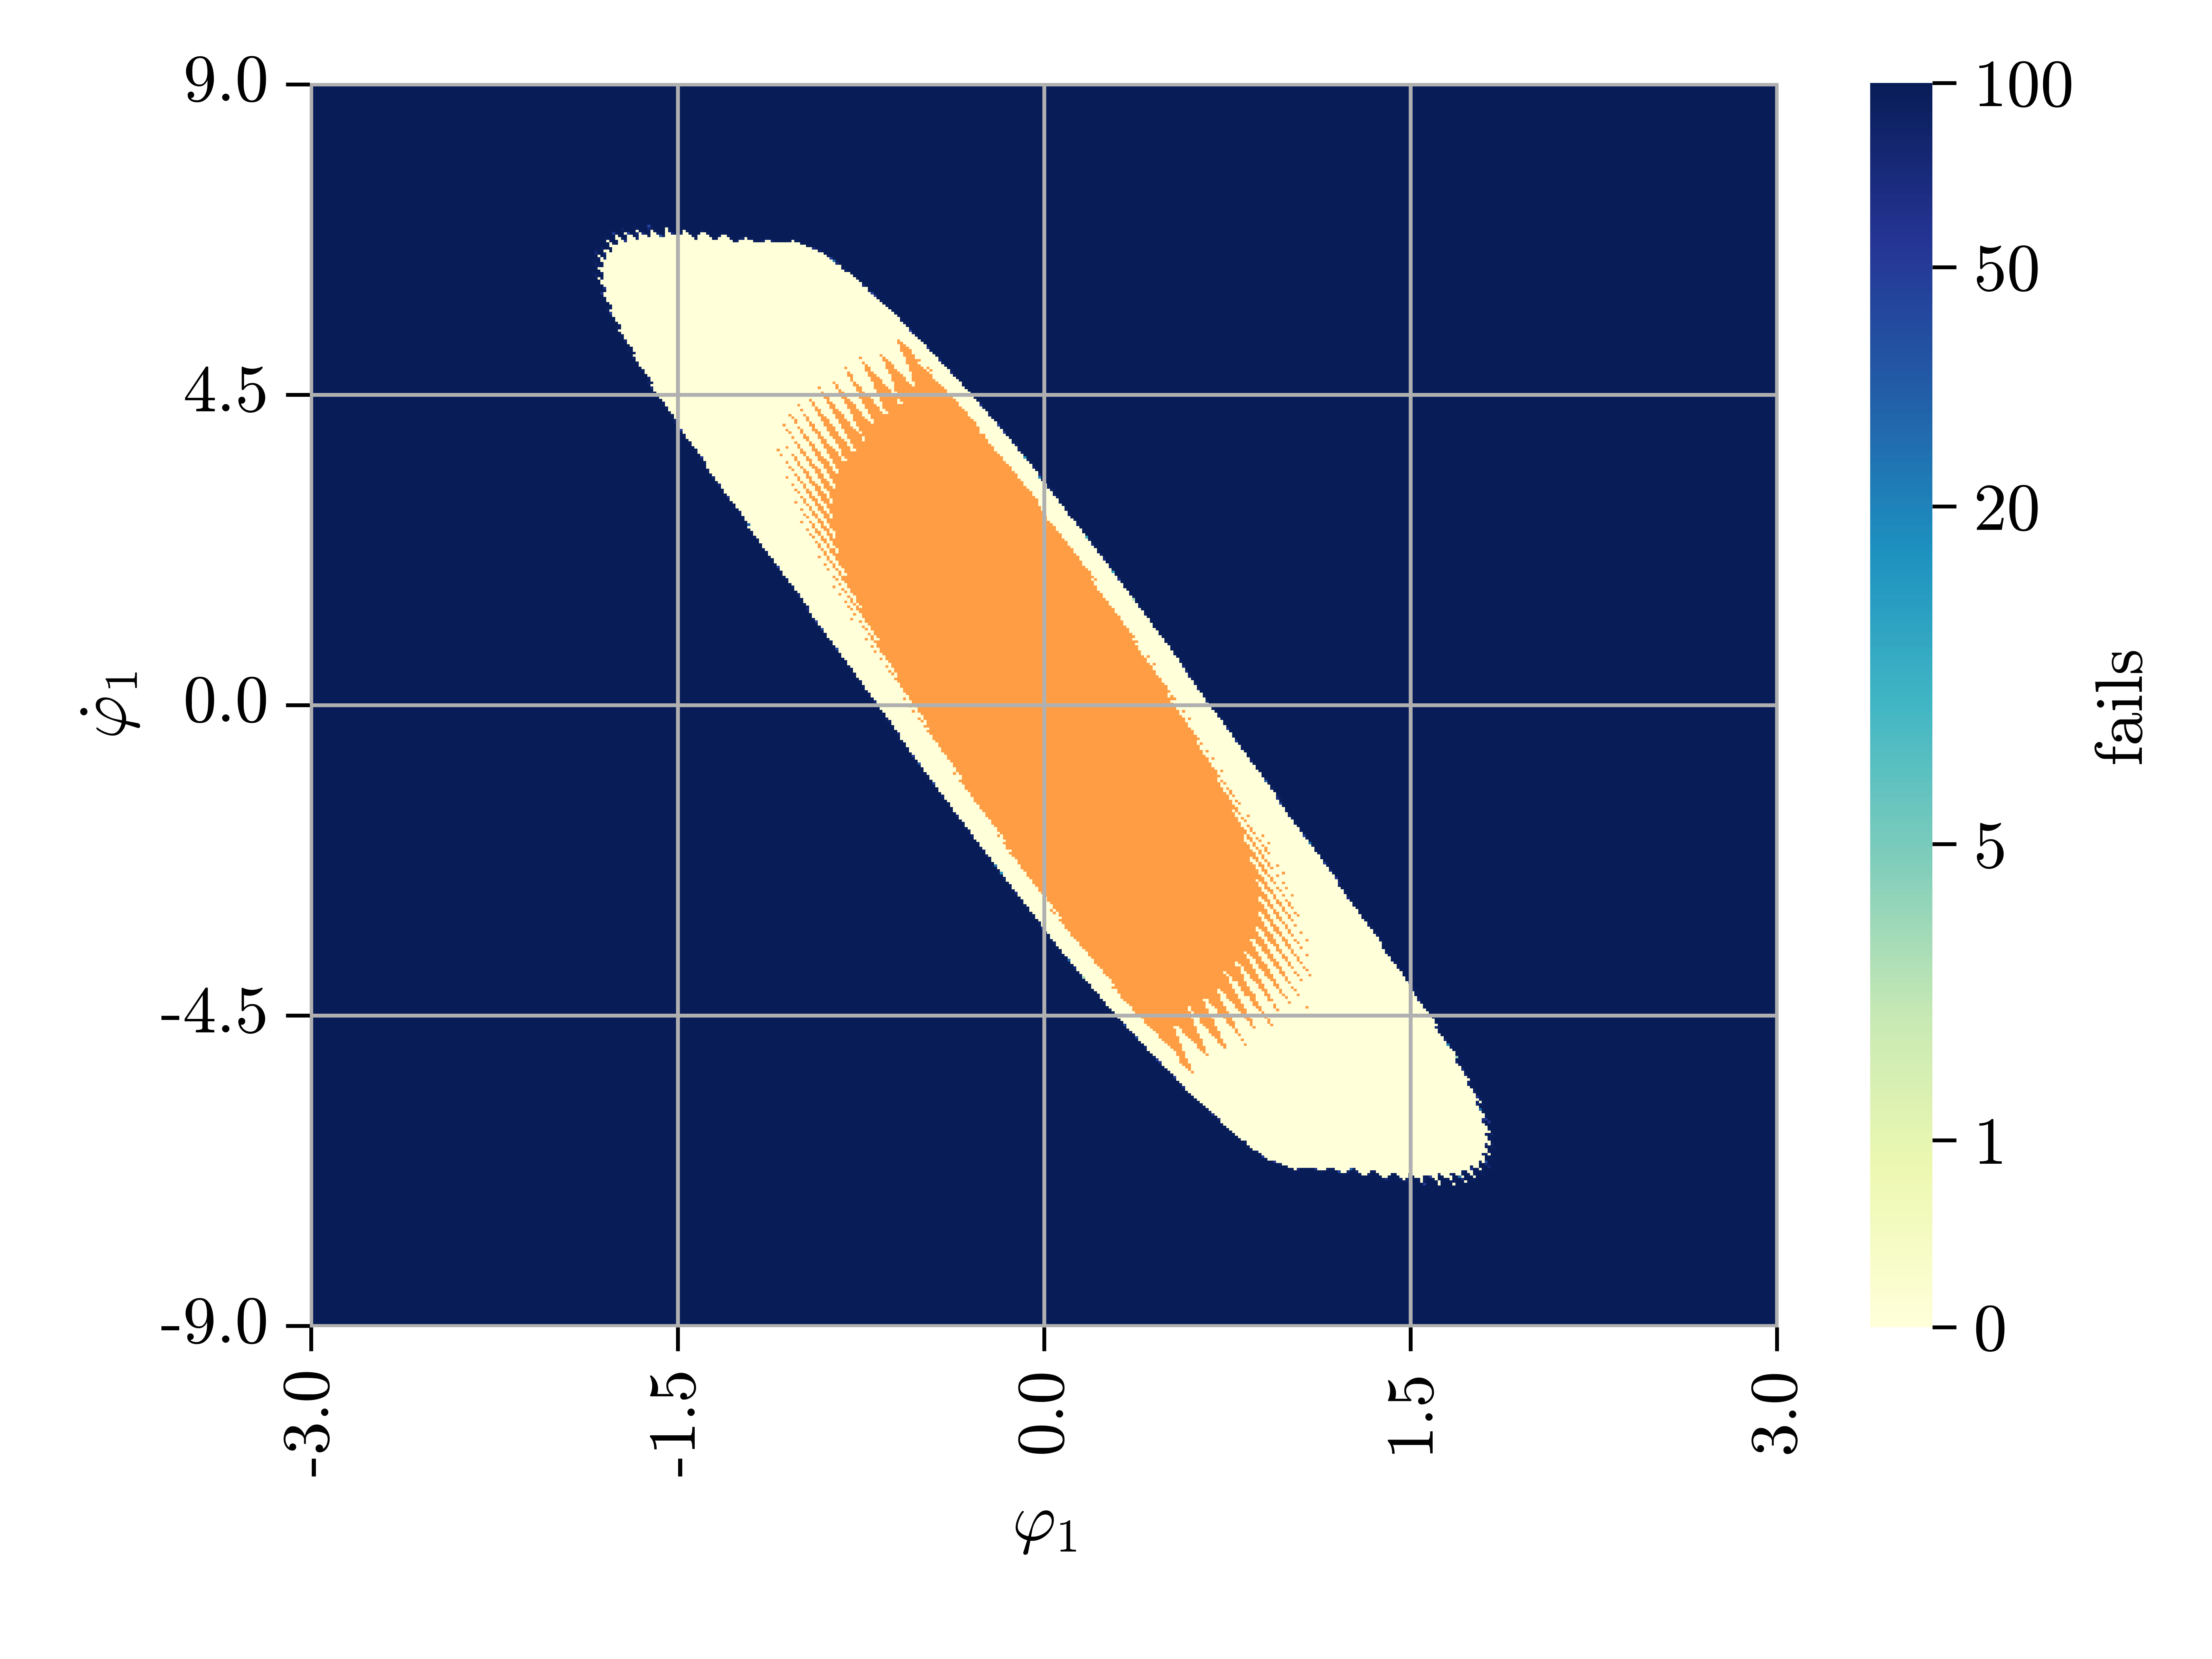
\includegraphics[width=\textwidth]{Figures/SP_continuous_vs_discrete_phi1phi1dot.png}
		\label{fig: sp - continuous vs discrete}
		\caption{}
	\end{subfigure}
	\hfill
	\begin{subfigure}[t]{0.48\textwidth}
		\centering
		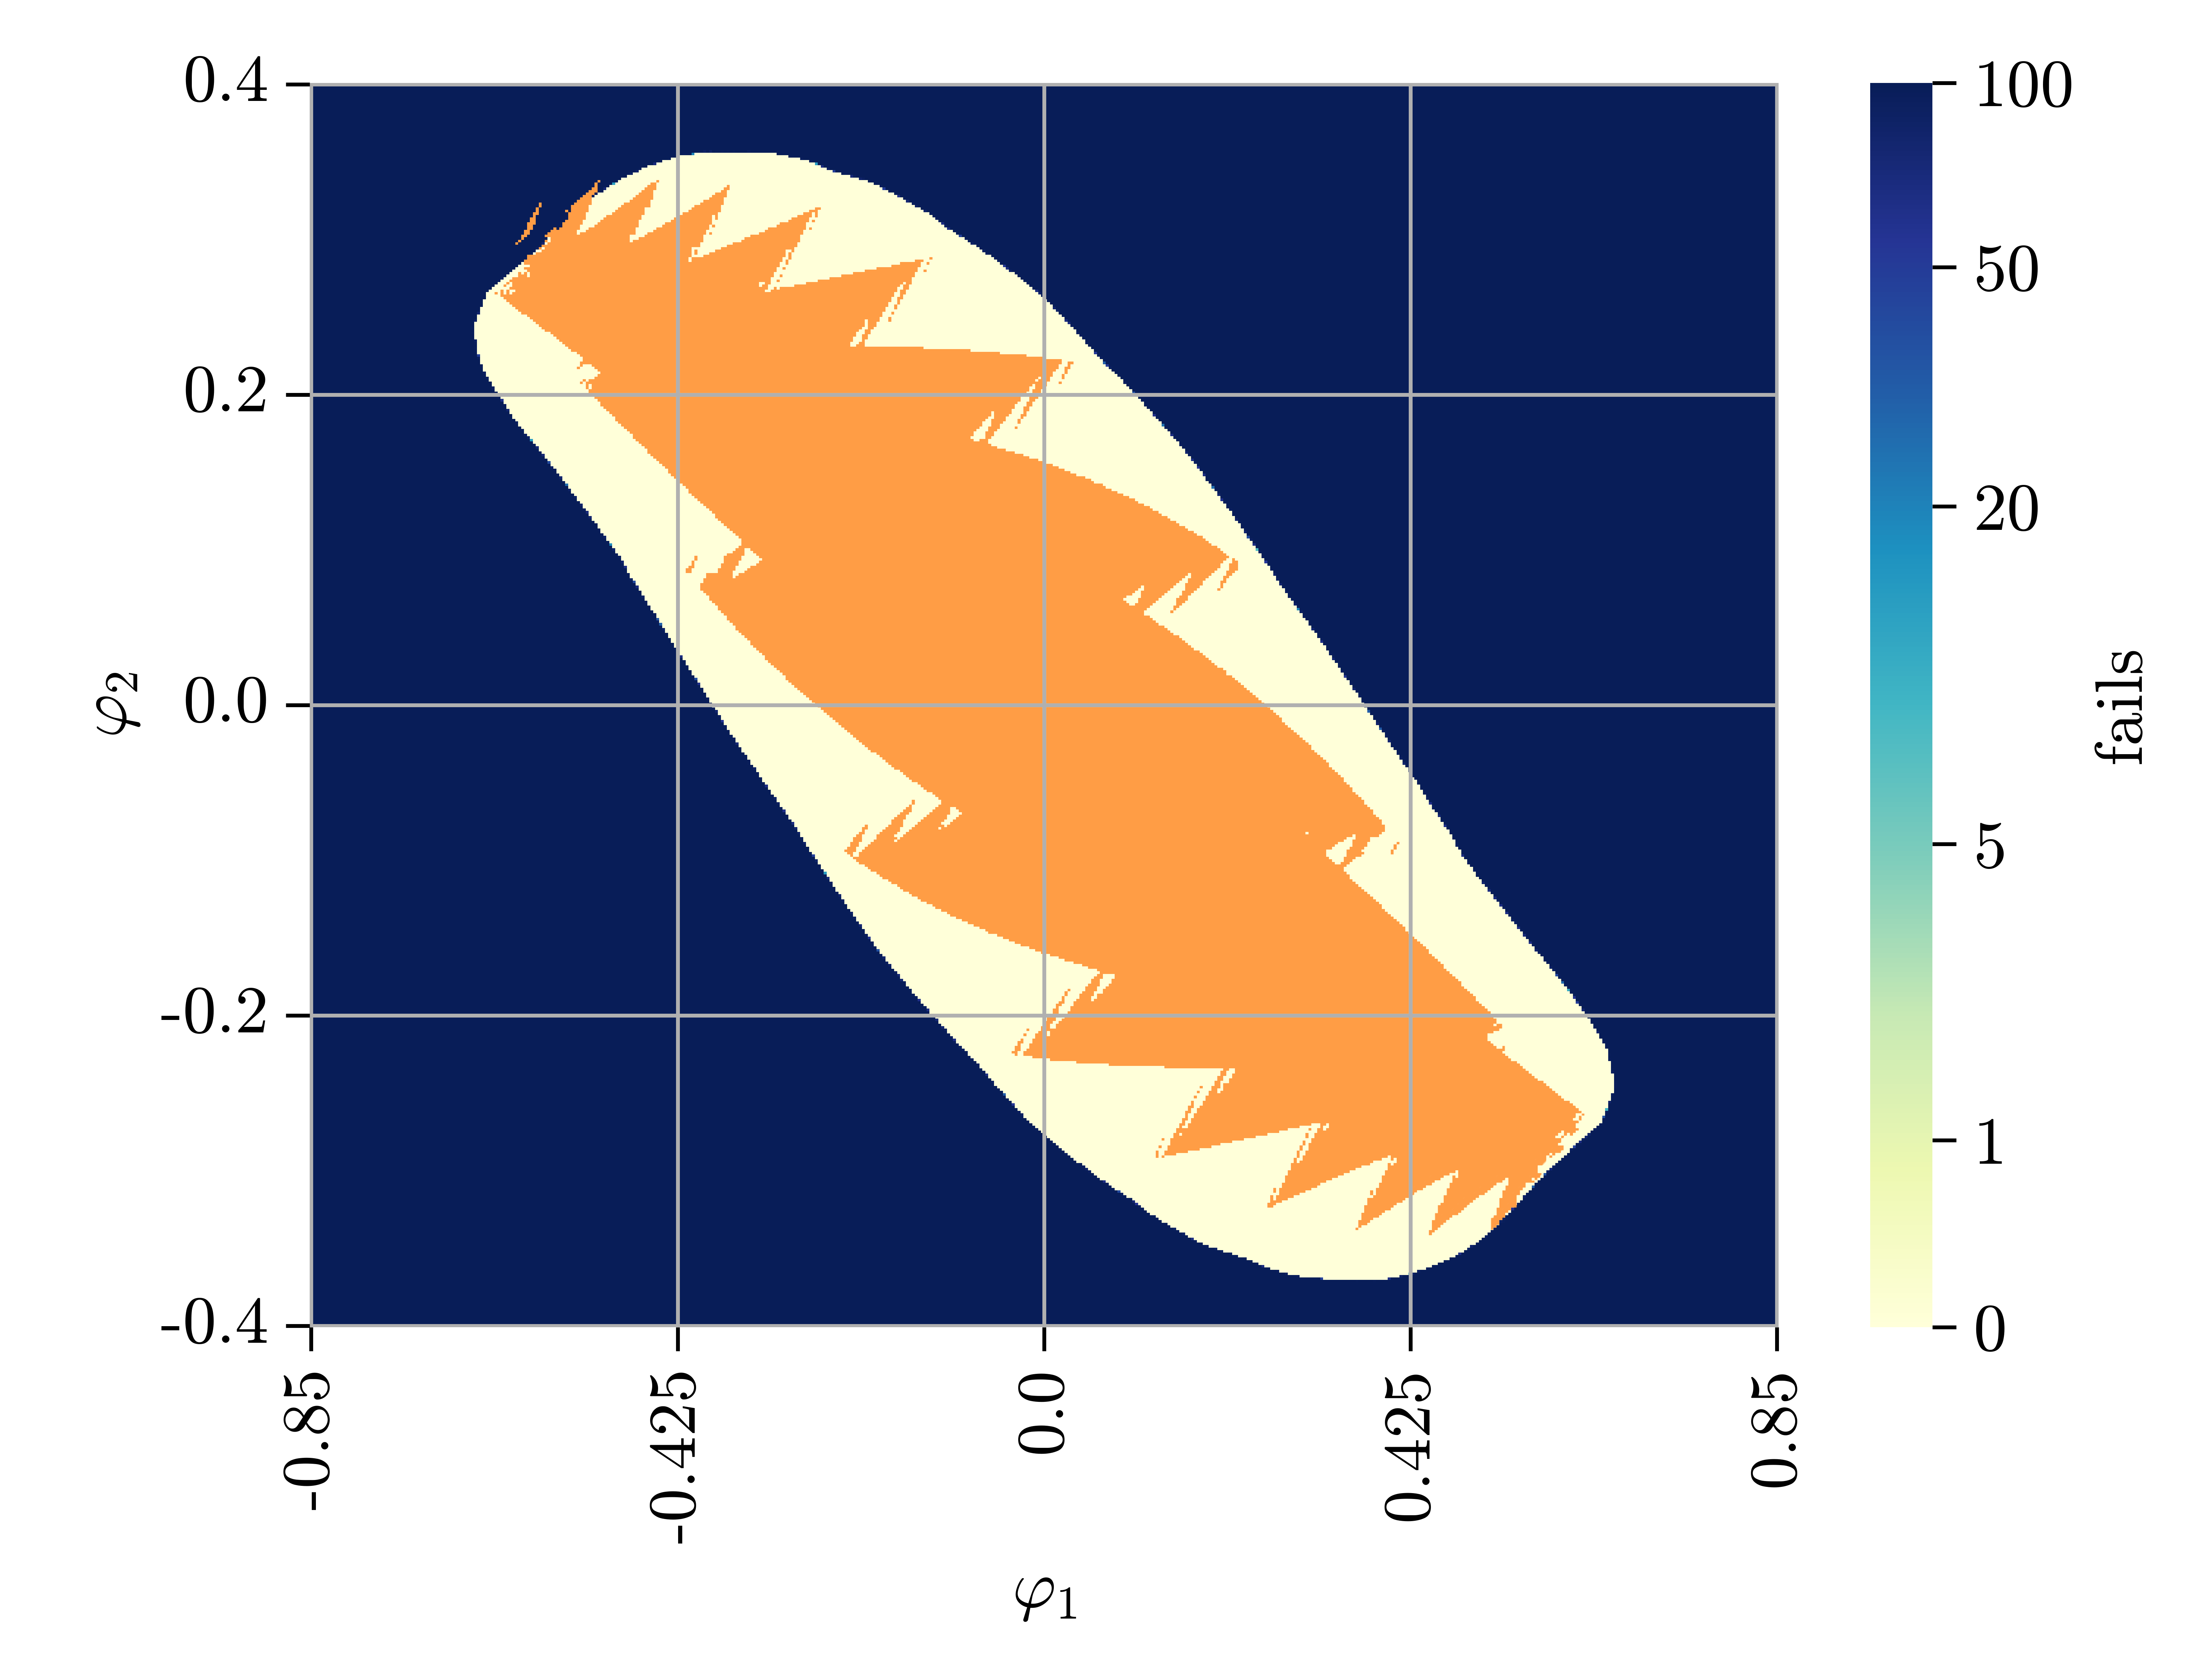
\includegraphics[width=\textwidth]{Figures/DP_continuous_vs_discrete_phi1phi2.png}
		\label{fig: dp - continuous vs discrete}
		\caption{}
	\end{subfigure}
	
	\vspace{0.2cm}
	
	\begin{subfigure}[t]{0.48\textwidth}
		\centering
		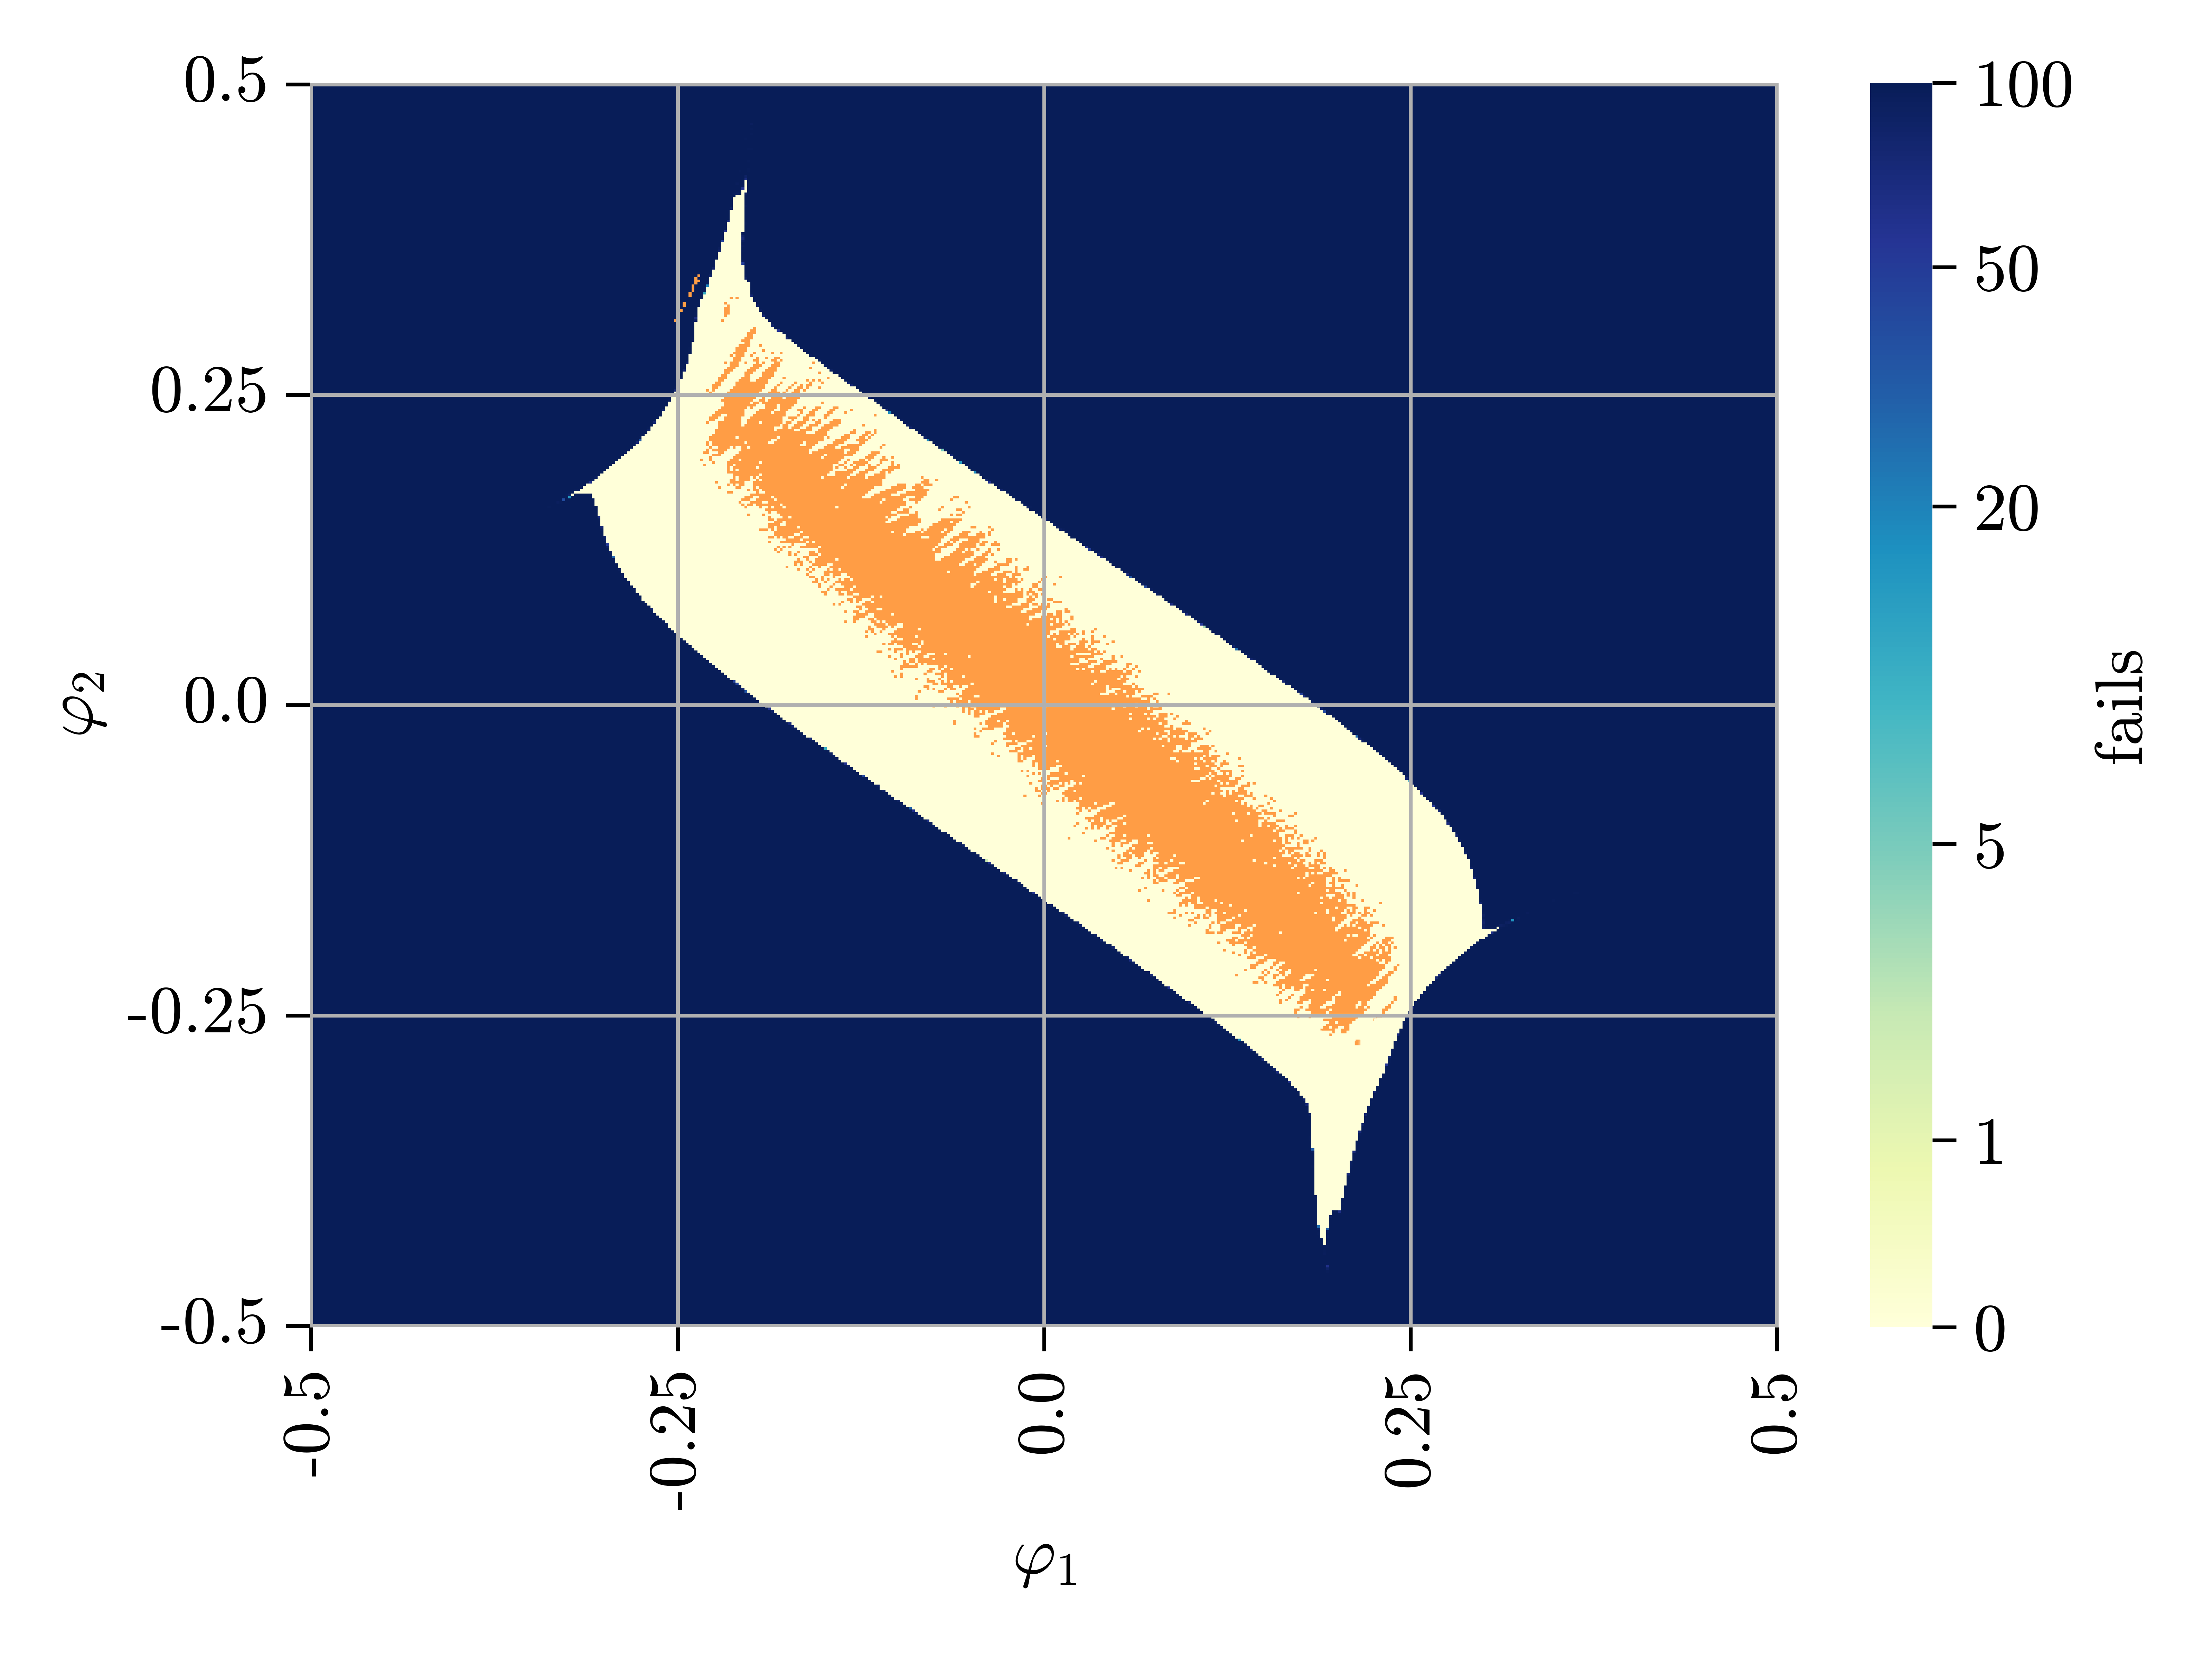
\includegraphics[width=\textwidth]{Figures/TP_continuous_vs_discrete_phi1phi2.png}
		\label{fig: tp - continuous vs discrete, phi1 phi2}
		\caption{}
	\end{subfigure}
	\hfill
	\begin{subfigure}[t]{0.48\textwidth}
		\centering
		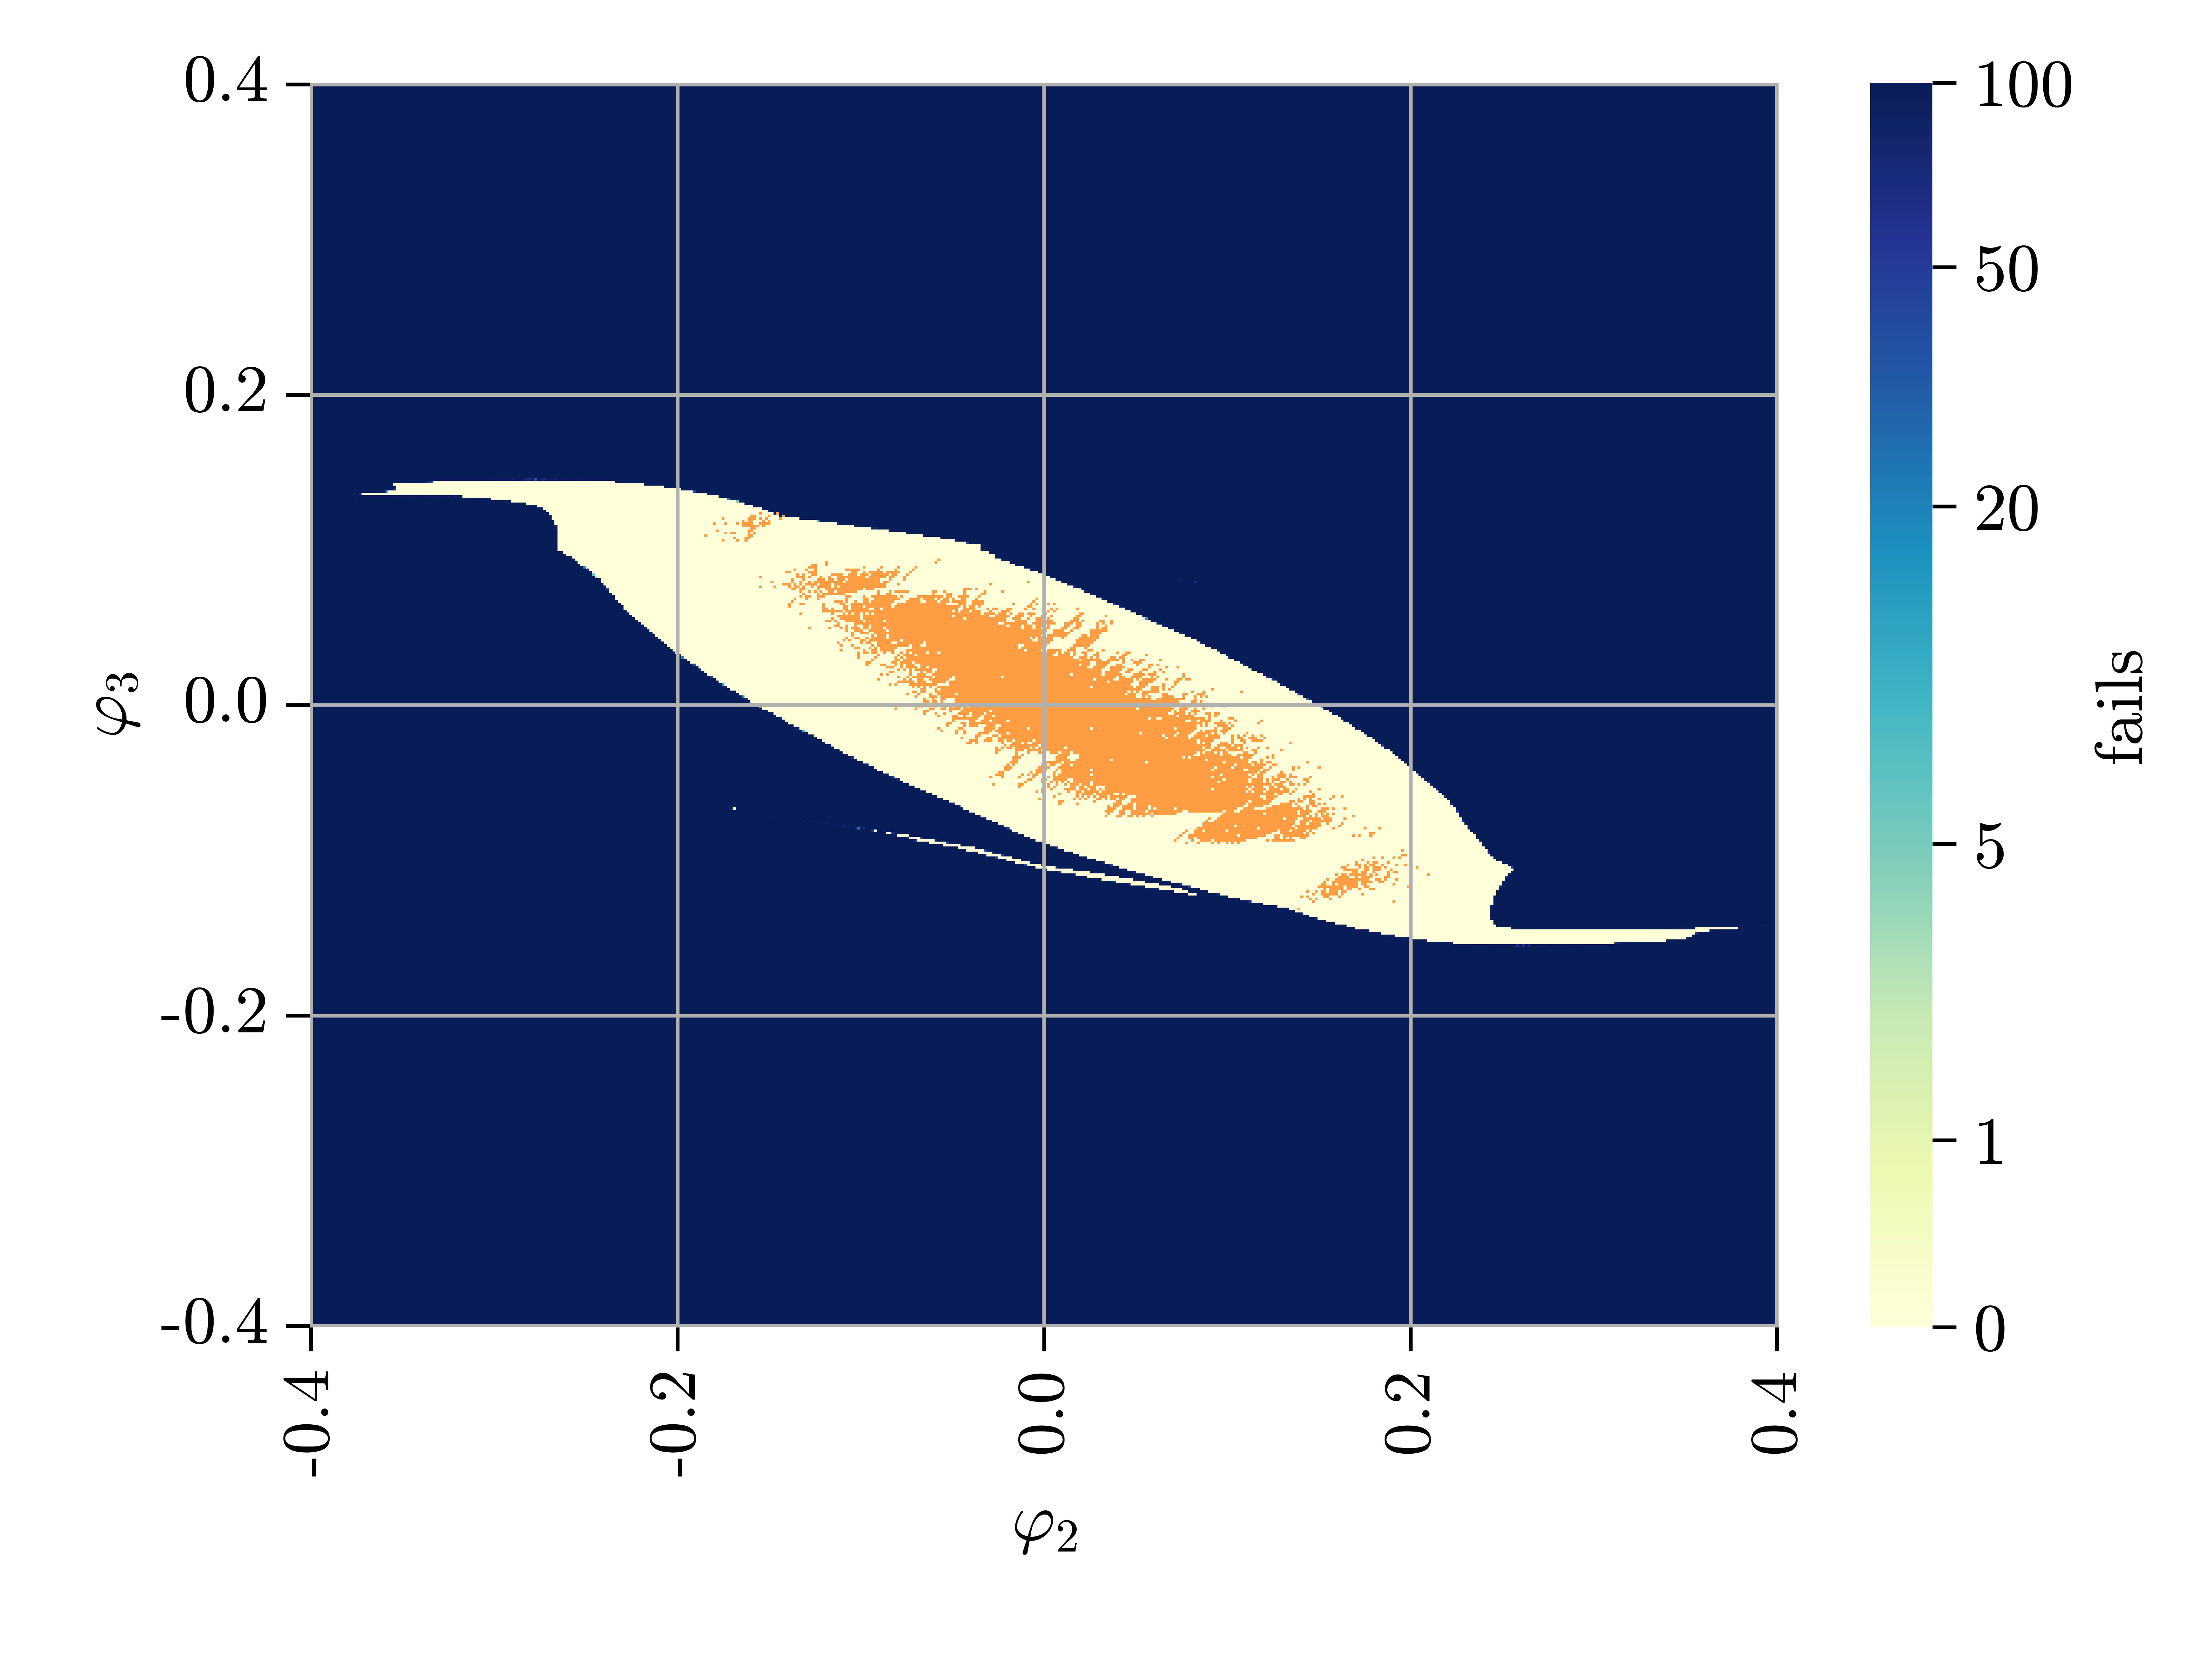
\includegraphics[width=\textwidth]{Figures/TP_continuous_vs_discrete_phi2phi3.png}
		\label{fig: tp - continuous vs discrete, phi2 phi3}
		\caption{}
	\end{subfigure}
	
	\caption{Stability zones comparison of the PPO agent using different control strategies. For the 1-link system (a) the zone axis are link's angle $\phi_1$ and angular velocity $\dot{\phi_1}$, while for the 2-link system (b) axis are the pendulum link angles $\phi_1$ and $\phi_2$. Figures (b) and (c) present the stability zones based on the dependence of pendulum link angles of $\phi_1$ and $\phi_2$ and of $\phi_2$ and $\phi_3$. The discrete control stability zone is indicated in orange; continuous is in white beige. Each grid cell represents 100 randomized tests.}
	\label{fig: continuous vs discrete}
\end{figure}

The training speed is also significantly different in terms of reaching the required amount of tests for the discrete and continuous control algorithm while it is not clearly seen for the 1- and 2-link systems. Comparison of it is shown at the Fig~\ref{fig: training time comparison}. To clarify what trains faster, the line, where the agent reaches maximum required amount of successful tests is drawn for each system with the shown time step. For all three cases the difference between the discrete and continuous control algorithm is around 45-50$\%$ in reaching the successful training, while for the triple pendulum the stable training using discrete control algorithm has be reached after 500 000 time steps.  

\begin{figure}[h!]
	\centering
	\begin{subfigure}[t]{0.48\textwidth}
		\centering
		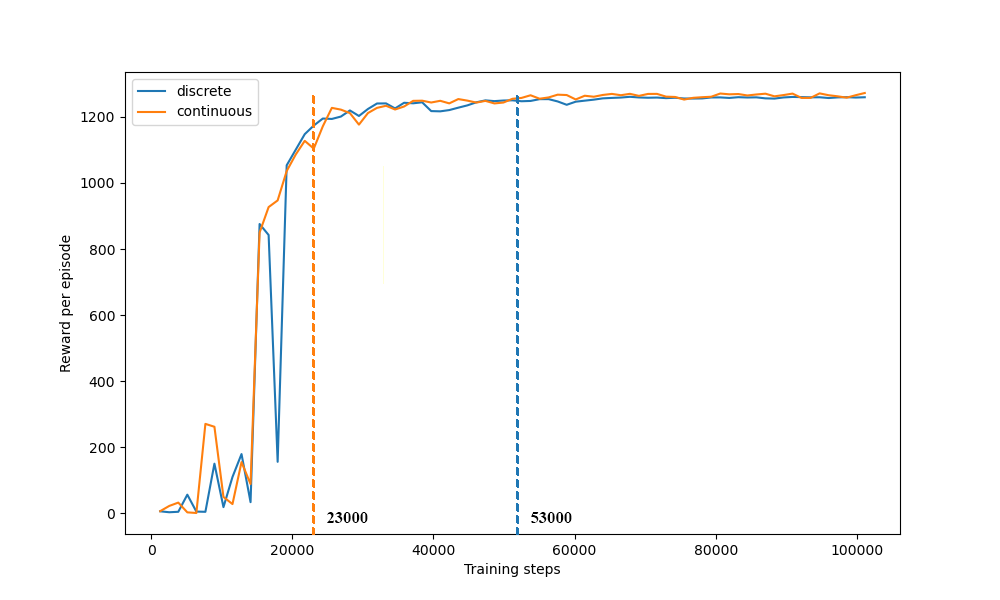
\includegraphics[width=\textwidth]{Figures/SP_discrete_vs_continuous_training_time.png}
		\label{fig: sp - training time}
		\caption{}
	\end{subfigure}
	\hfill
	\begin{subfigure}[t]{0.48\textwidth}
		\centering
		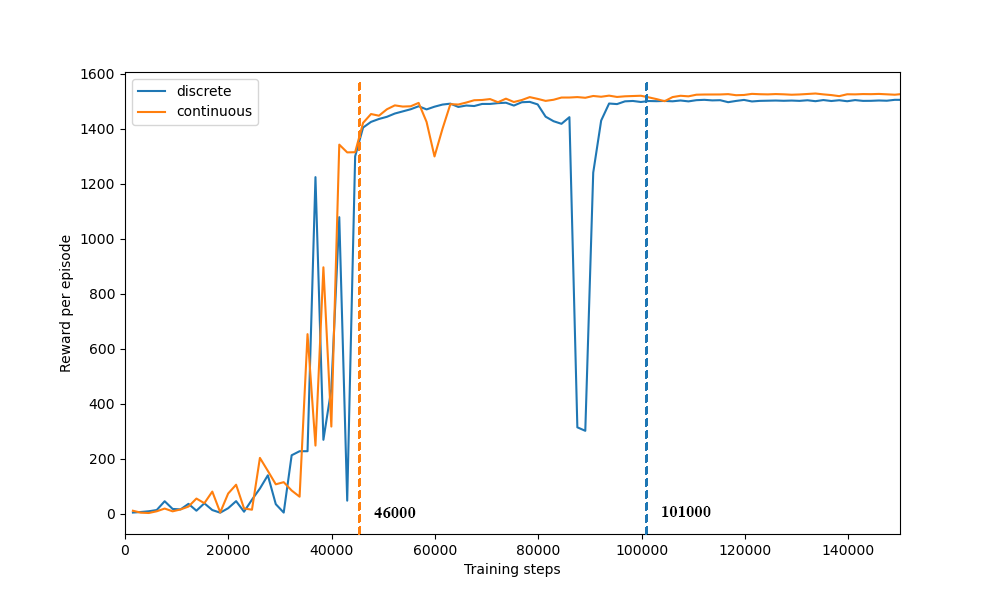
\includegraphics[width=\textwidth]{Figures/DP_discrete_vs_continuous_training_time.png}
		\label{fig: dp - training time}
		\caption{}
	\end{subfigure}
	\begin{subfigure}[t]{0.48\textwidth}
		\centering
		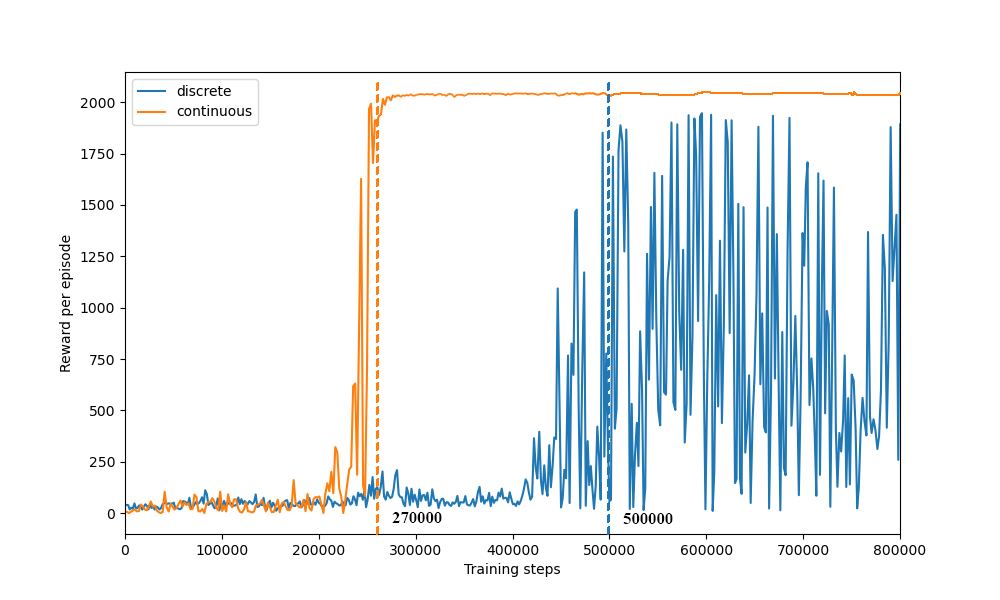
\includegraphics[width=\textwidth]{Figures/TP_discrete_vs_continuous_training_time.png}
		\label{fig: tp - training time}
		\caption{}
	\end{subfigure}
	
	\caption{Training times for the PPO agents for 1-link (a), 2-link (b) and 3-link (c) systems}
	\label{fig: training time comparison}
\end{figure}

Our results show, that not even the operating area of the RL agent is wider and smoother, but the agent also achieves a faster training result. 

\subsection{Agent tested on modified environments} \label{subsec: Agent tested on modified environments}
In this section, we examine the impact of changing properties of the environment, namely
link length, mass, and added friction, on the stability zones. The investigation is conducted
using the inverted double pendulum on a cart model (same continuous agent as in the Figure~\ref{fig: continuous vs discrete} (b)). In each subplot of Figure~\ref{fig: agent impact on different environments}, the stability zone is determined for the same agent in various modified environments, and the contour of the stability zone from the original environment is overlaid. Friction is implemented using the same method as in our previous research~\cite{manzl2023relrl}.

 \begin{figure}[h!]
     \centering
     \begin{subfigure}[t]{0.32\textwidth}
         \centering
         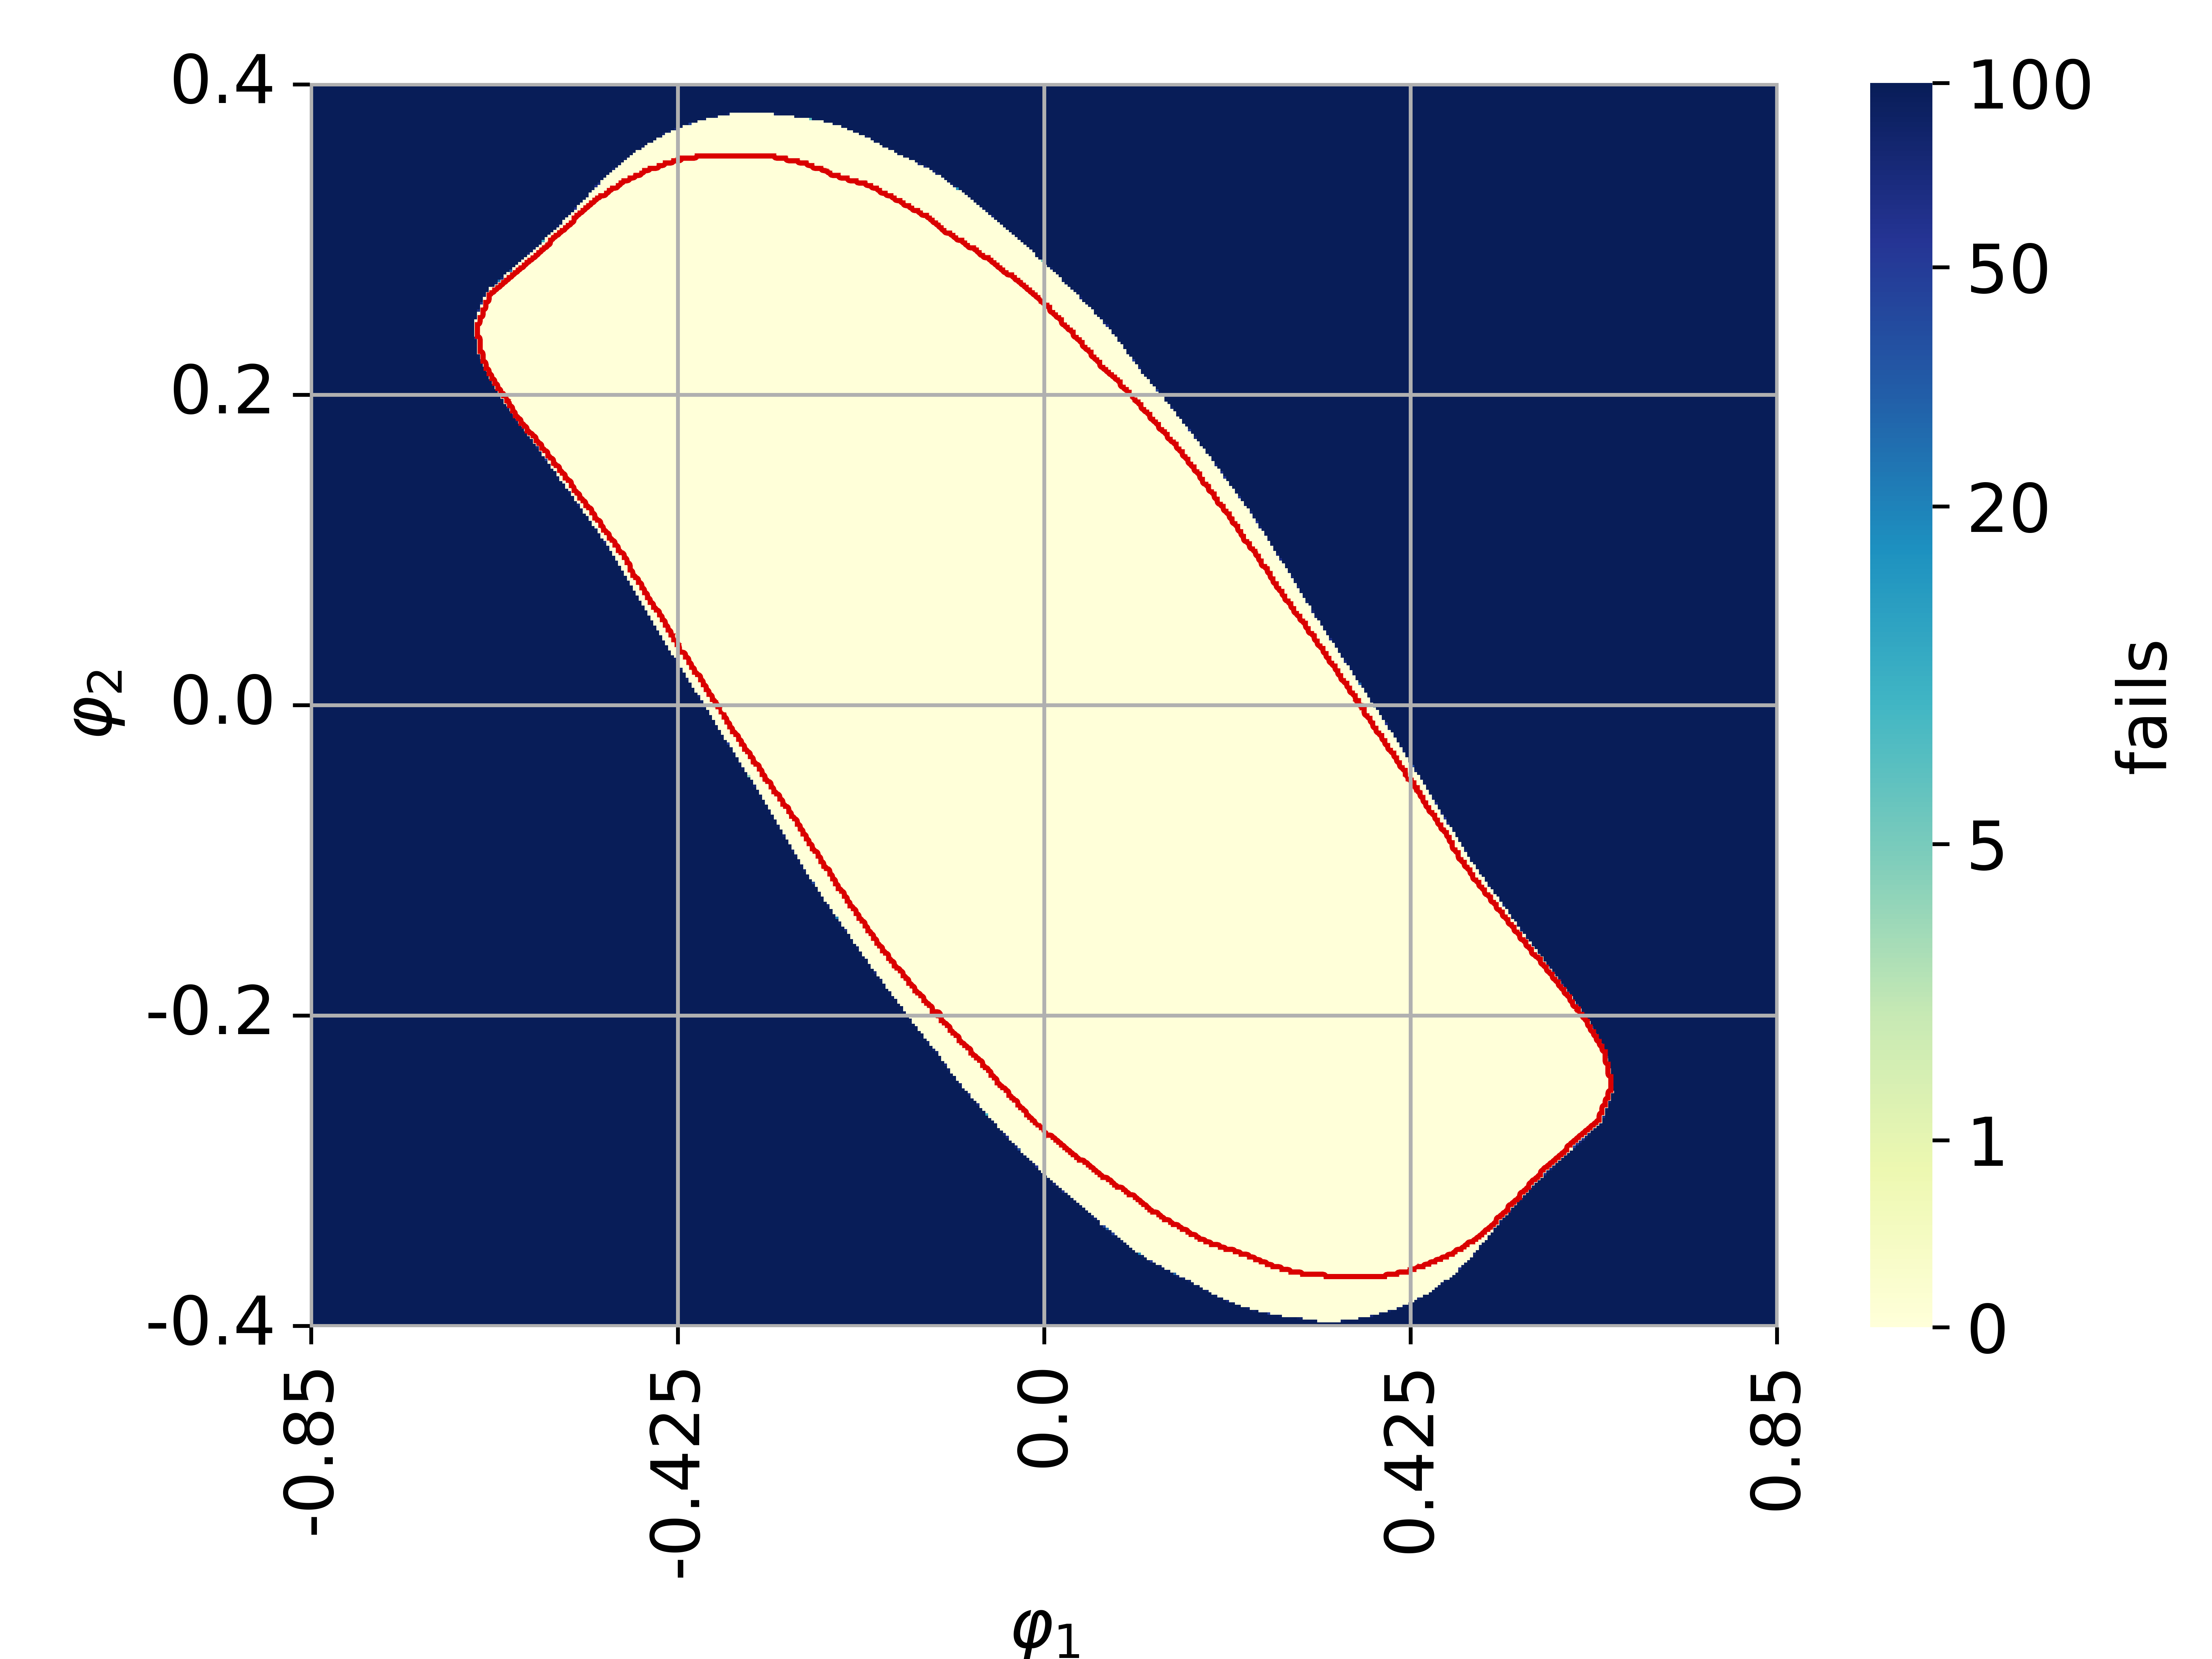
\includegraphics[width=\textwidth]{Figures/DP_len_1.1.png}
         \label{fig: DP len 1.1}
         \caption{}
     \end{subfigure}
     \hfill
     \begin{subfigure}[t]{0.32\textwidth}
         \centering
         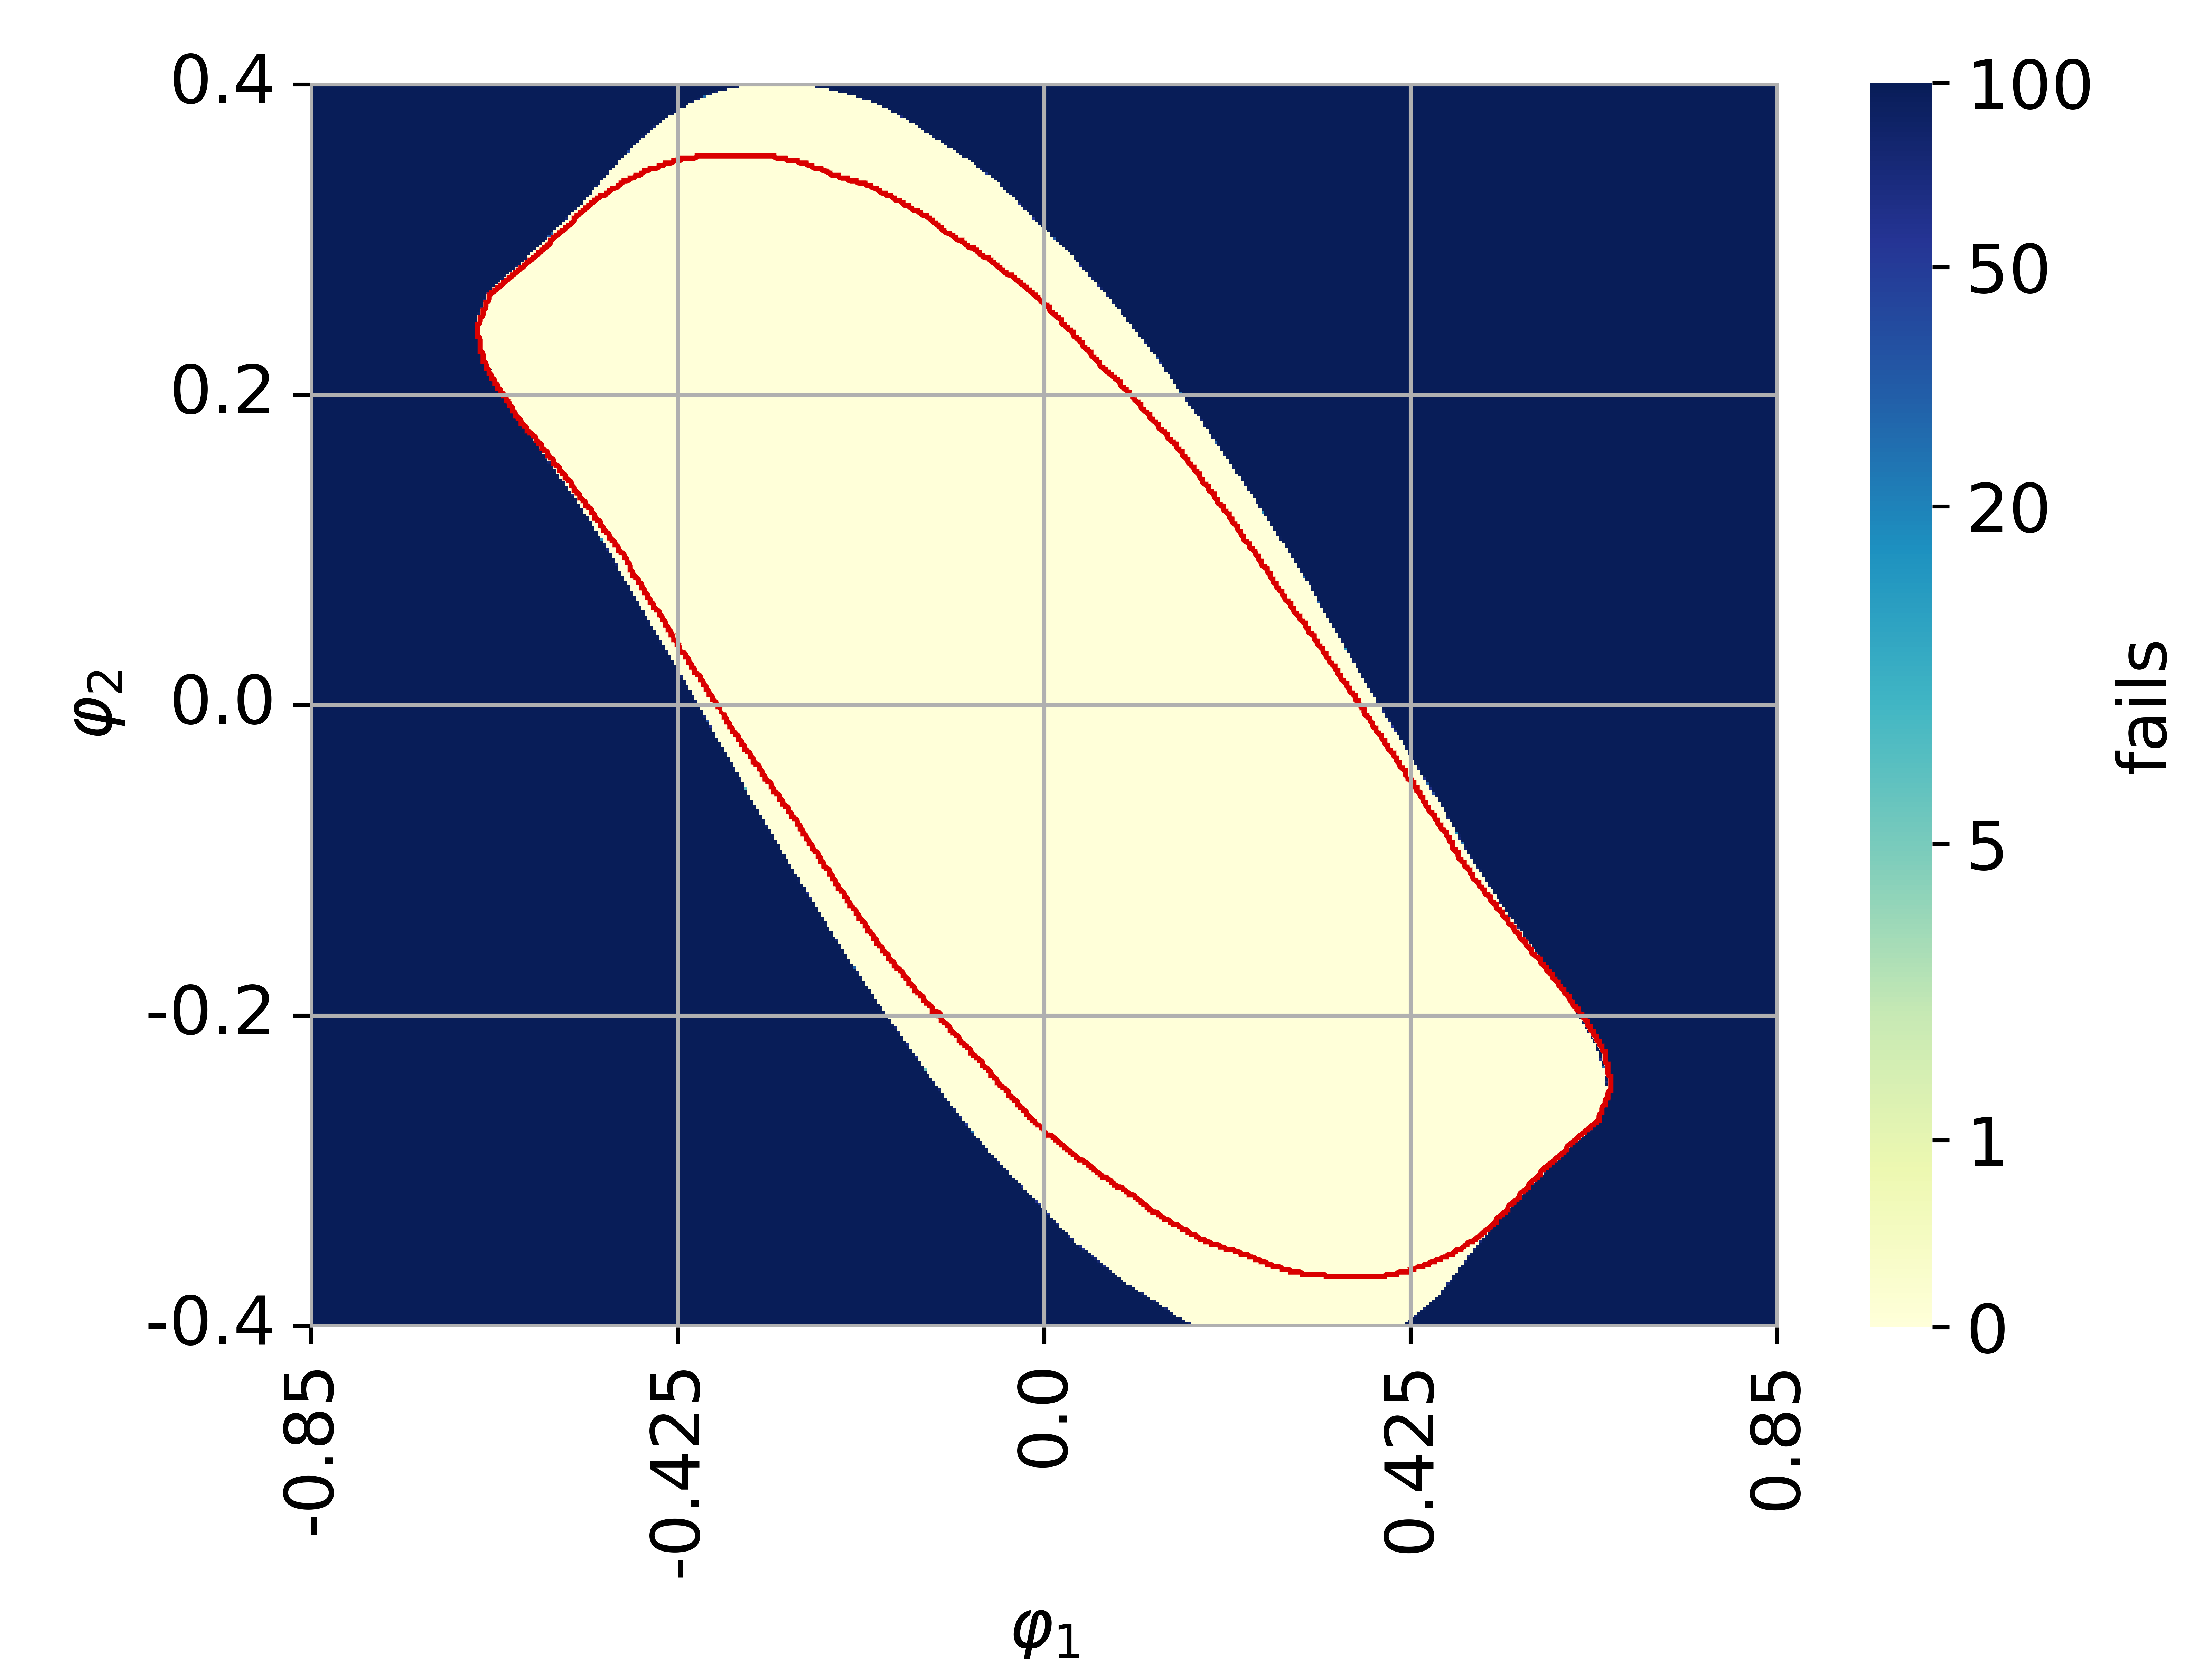
\includegraphics[width=\textwidth]{Figures/DP_len_1.2.png}
         \label{fig: DP len 1.2}
         \caption{}
     \end{subfigure}
     \hfill
     \begin{subfigure}[t]{0.32\textwidth}
         \centering
         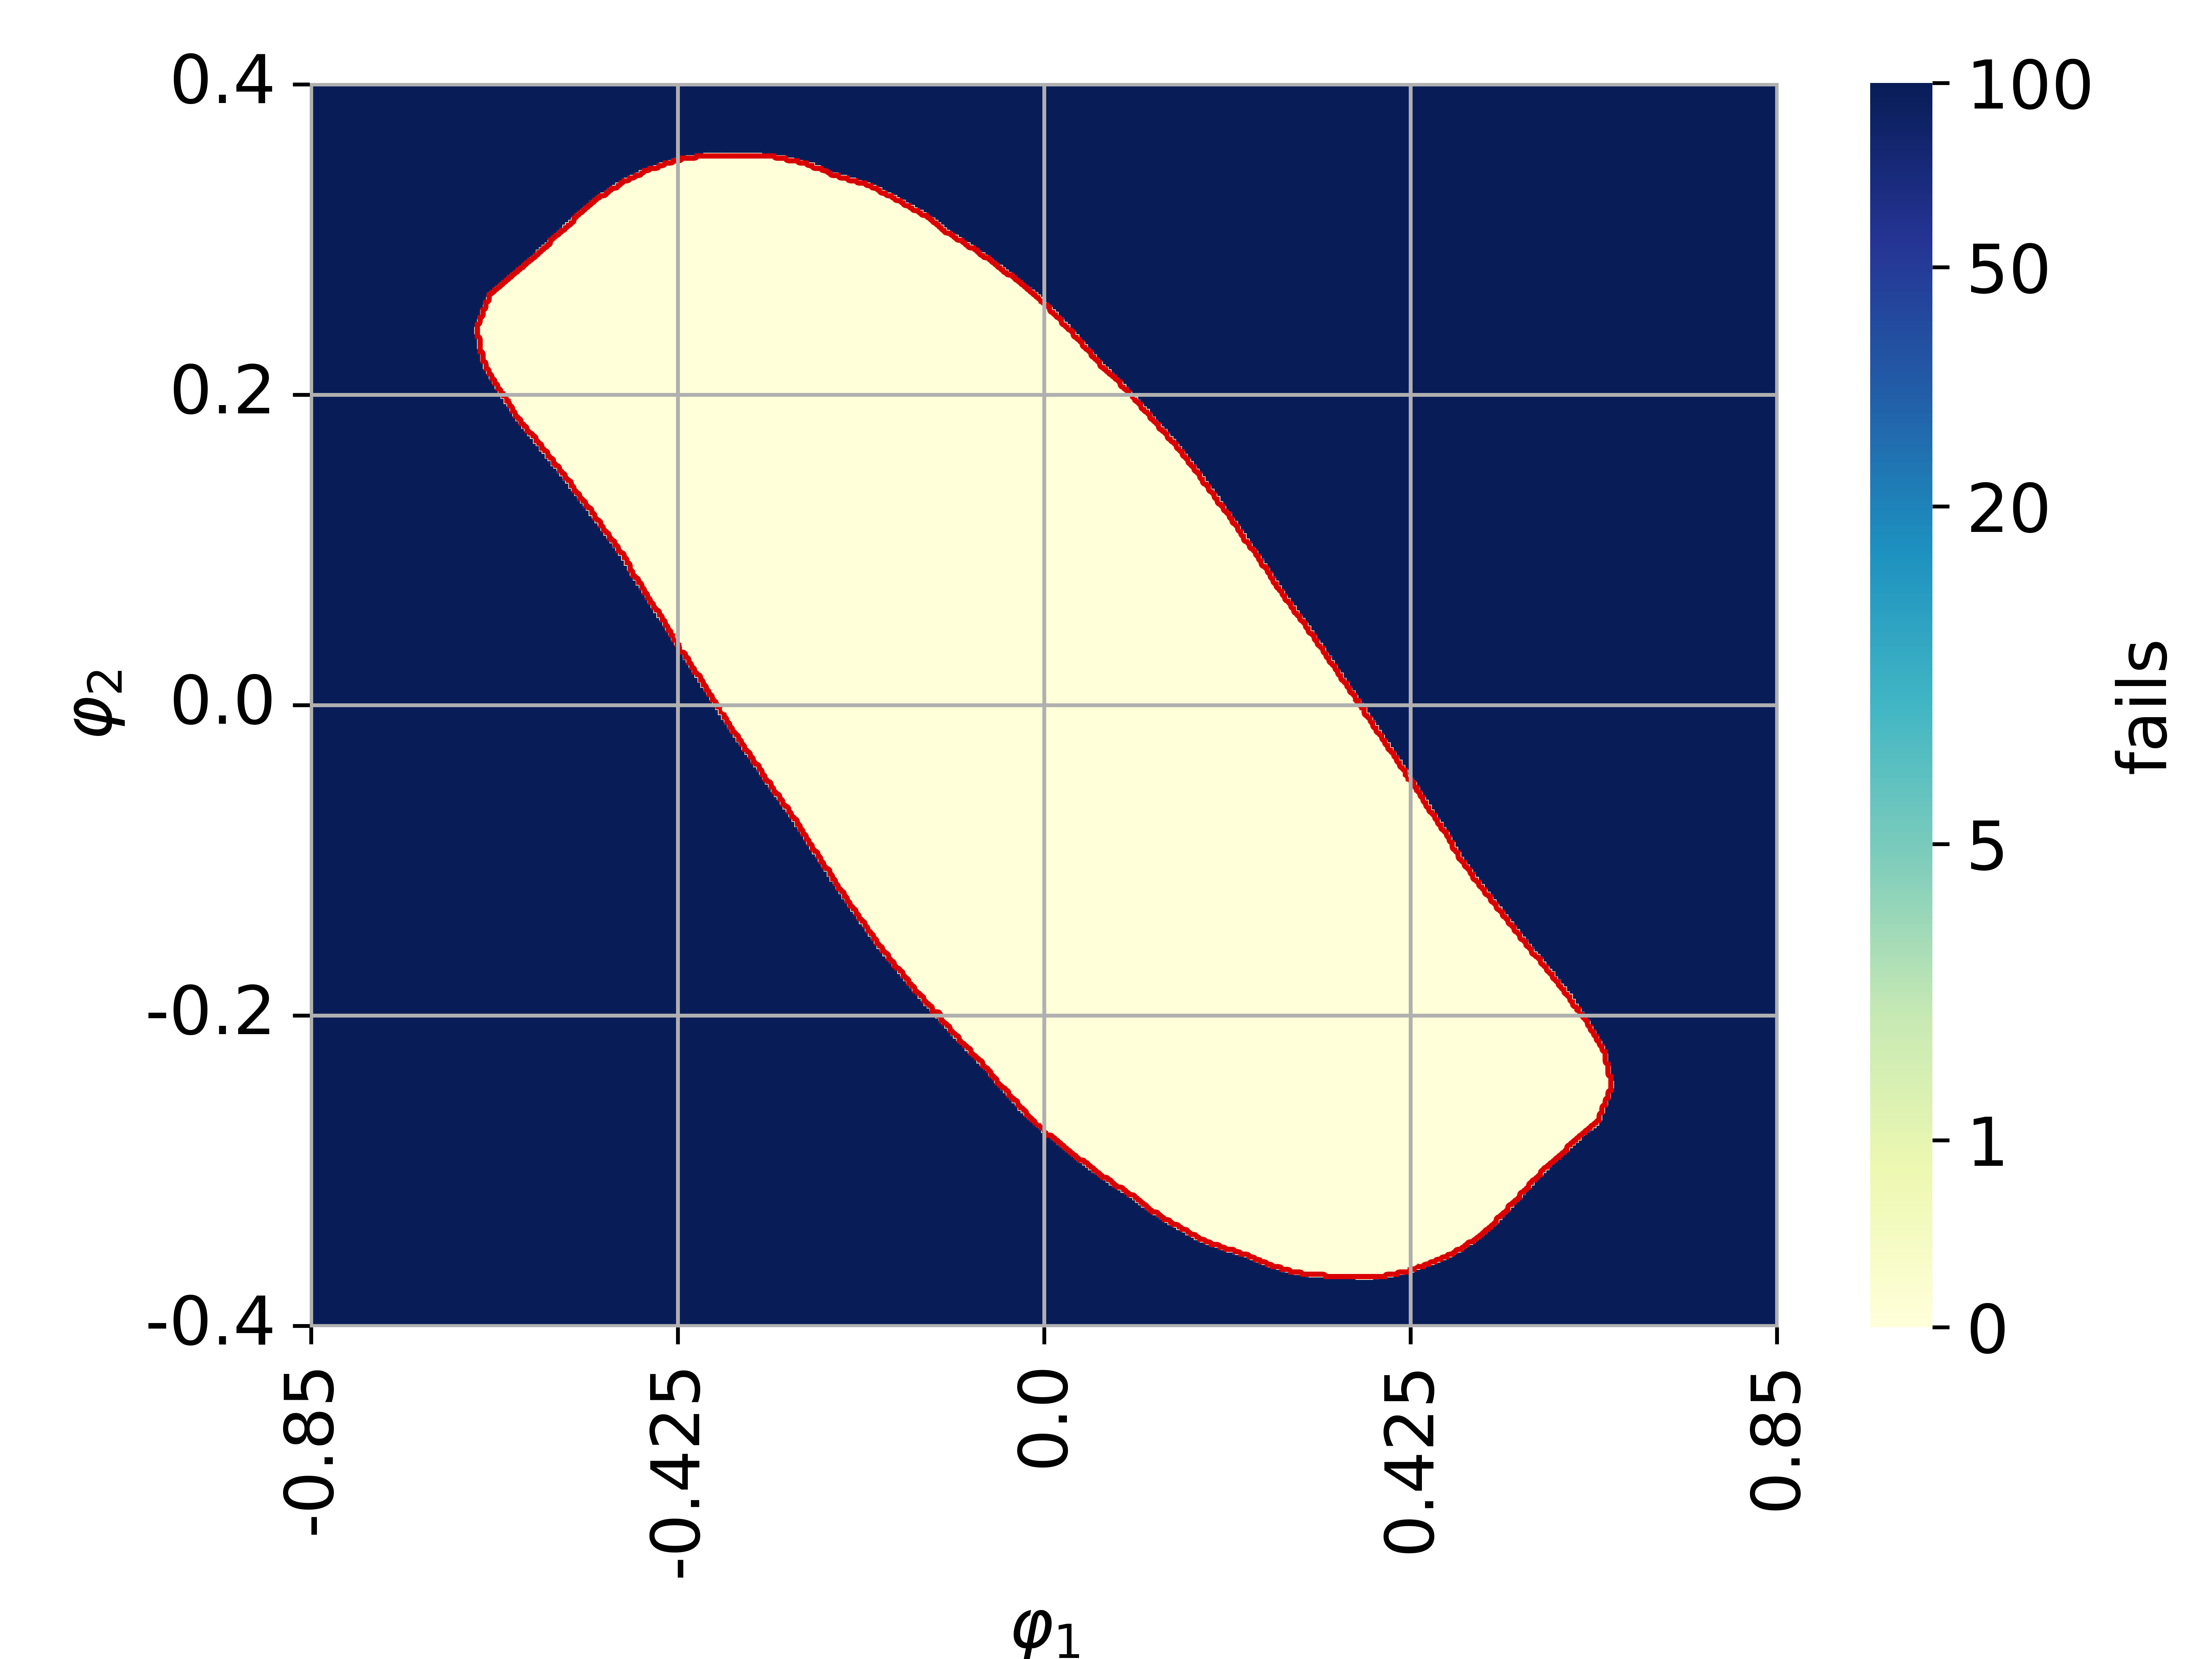
\includegraphics[width=\textwidth]{Figures/DP_mass_1.1.png}
         \label{fig: DP mass 1.1}
         \caption{}
     \end{subfigure}

     \vspace{0.2cm}

     \begin{subfigure}[t]{0.32\textwidth}
         \centering
         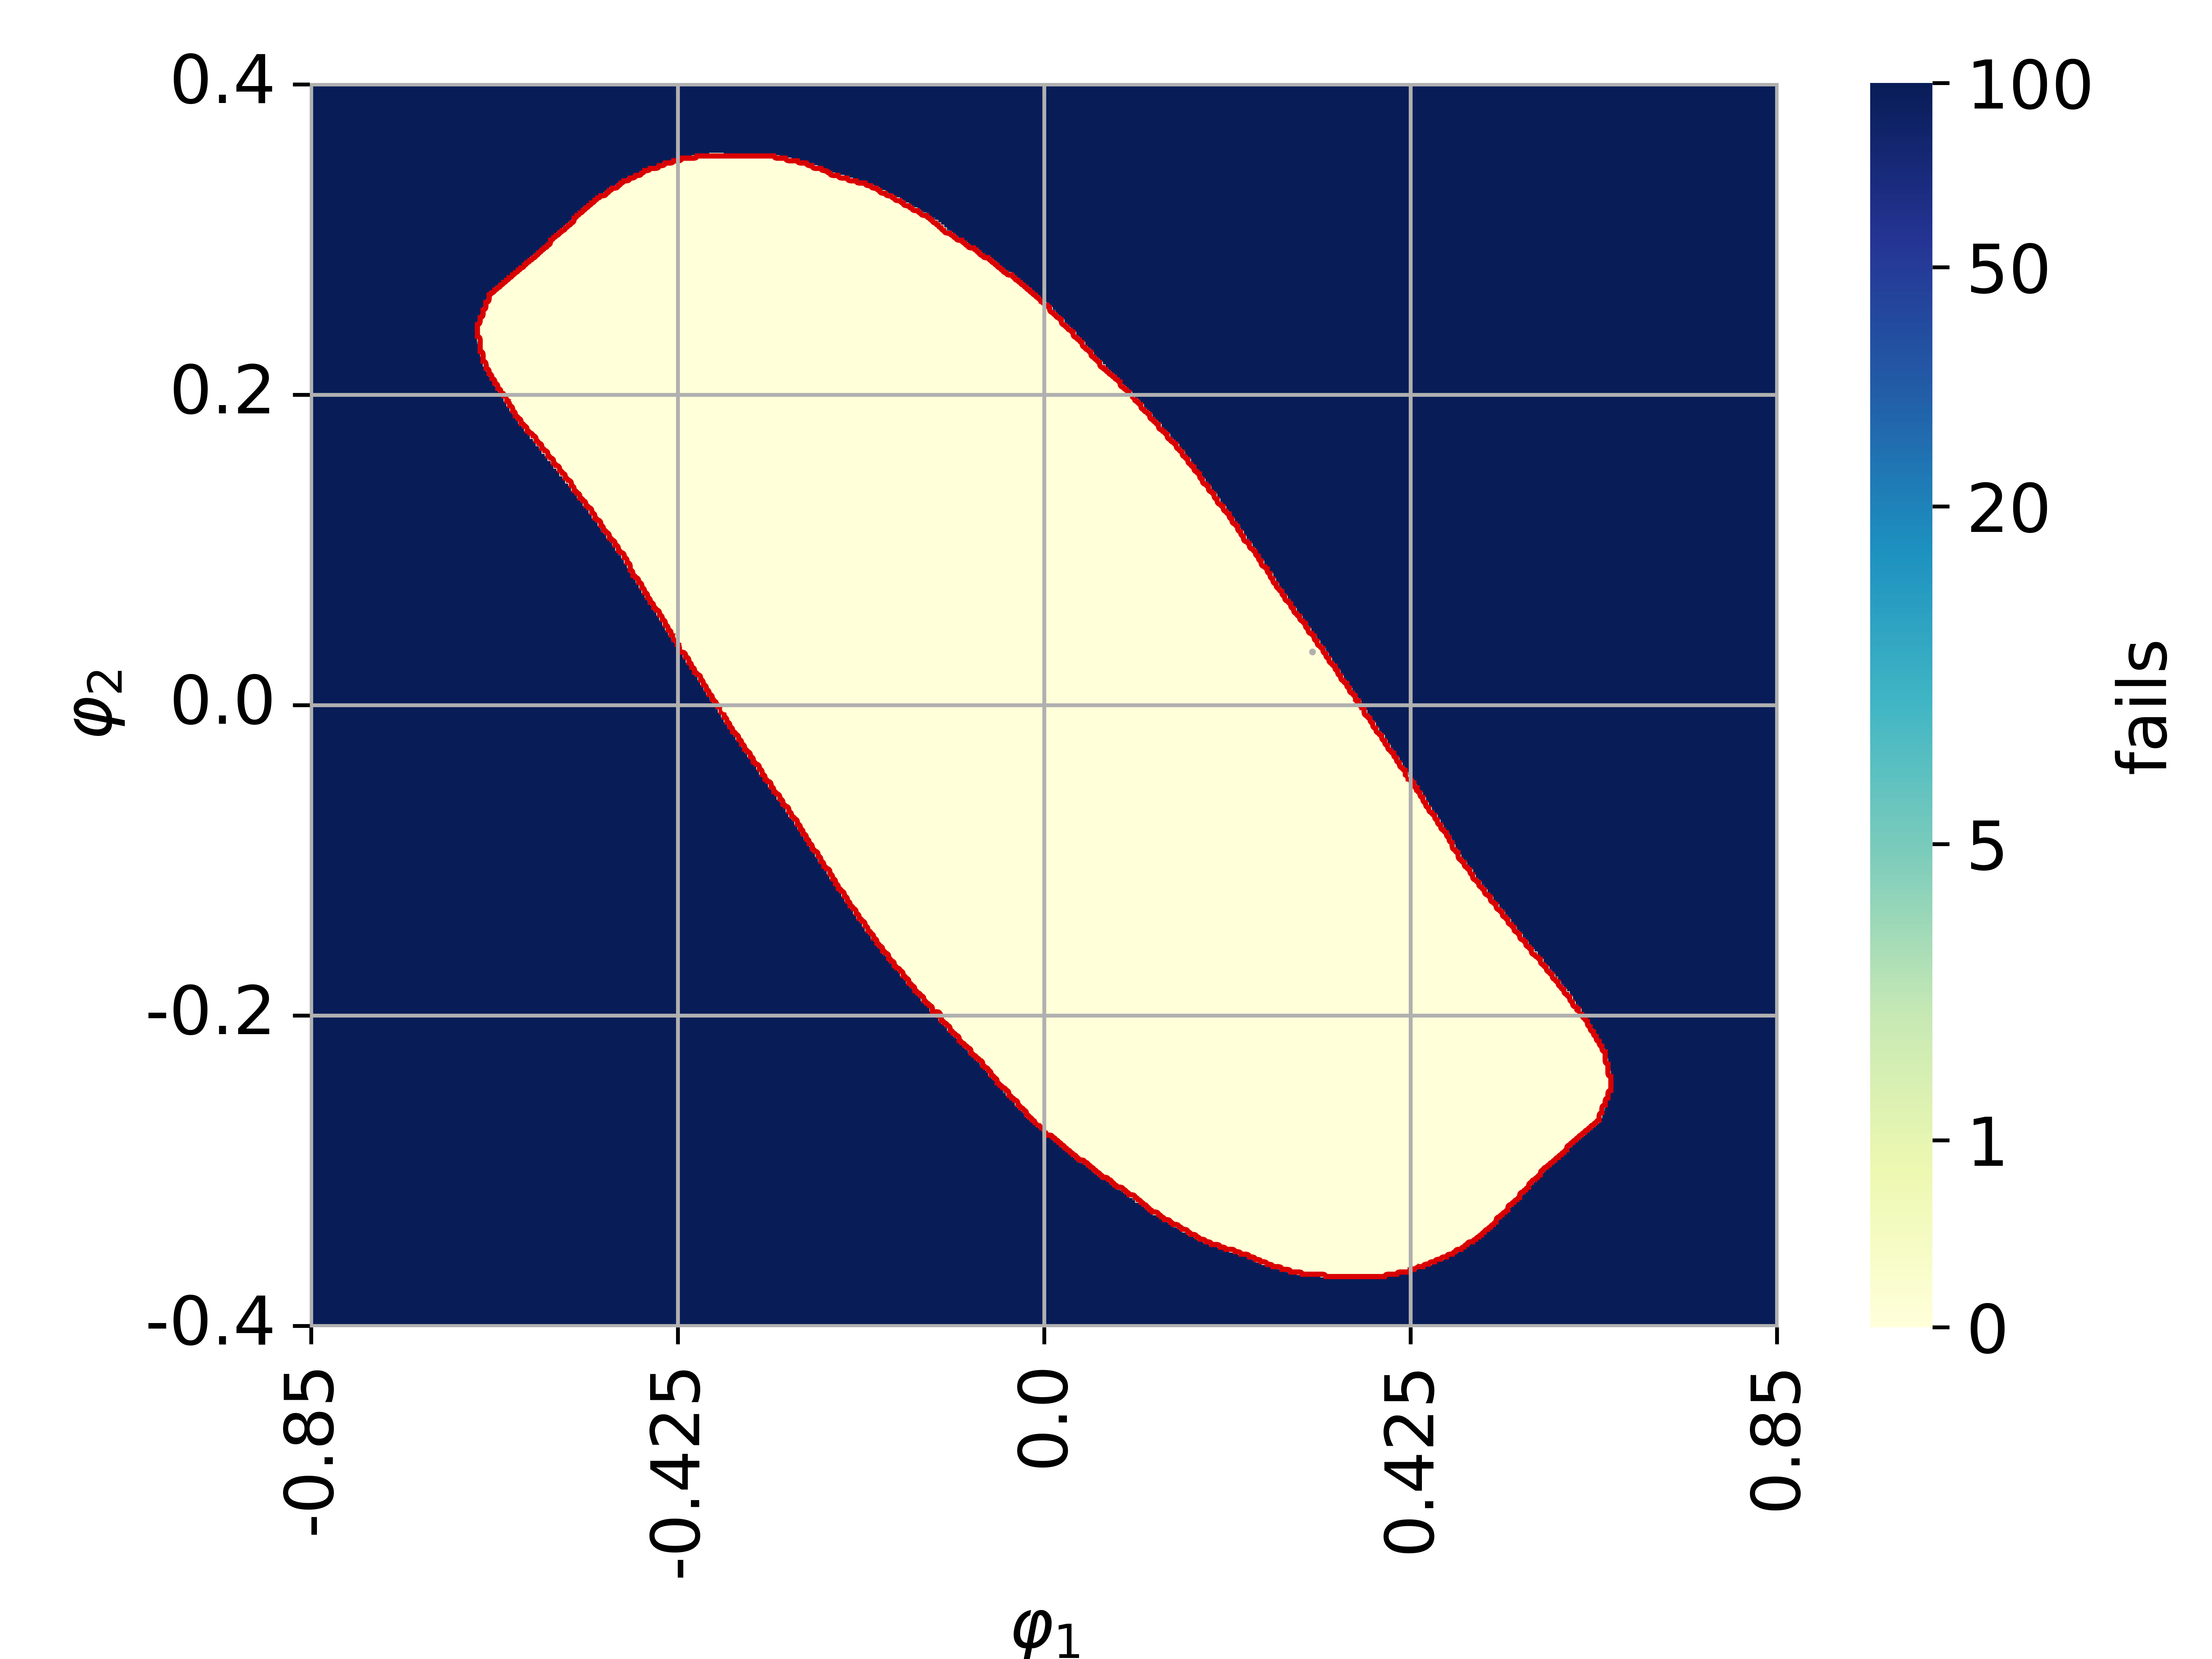
\includegraphics[width=\textwidth]{Figures/DP_mass_1.2.png}
         \label{fig: DP mass 1.2}
         \caption{}
     \end{subfigure}
     \hfill
     \begin{subfigure}[t]{0.32\textwidth}
         \centering
         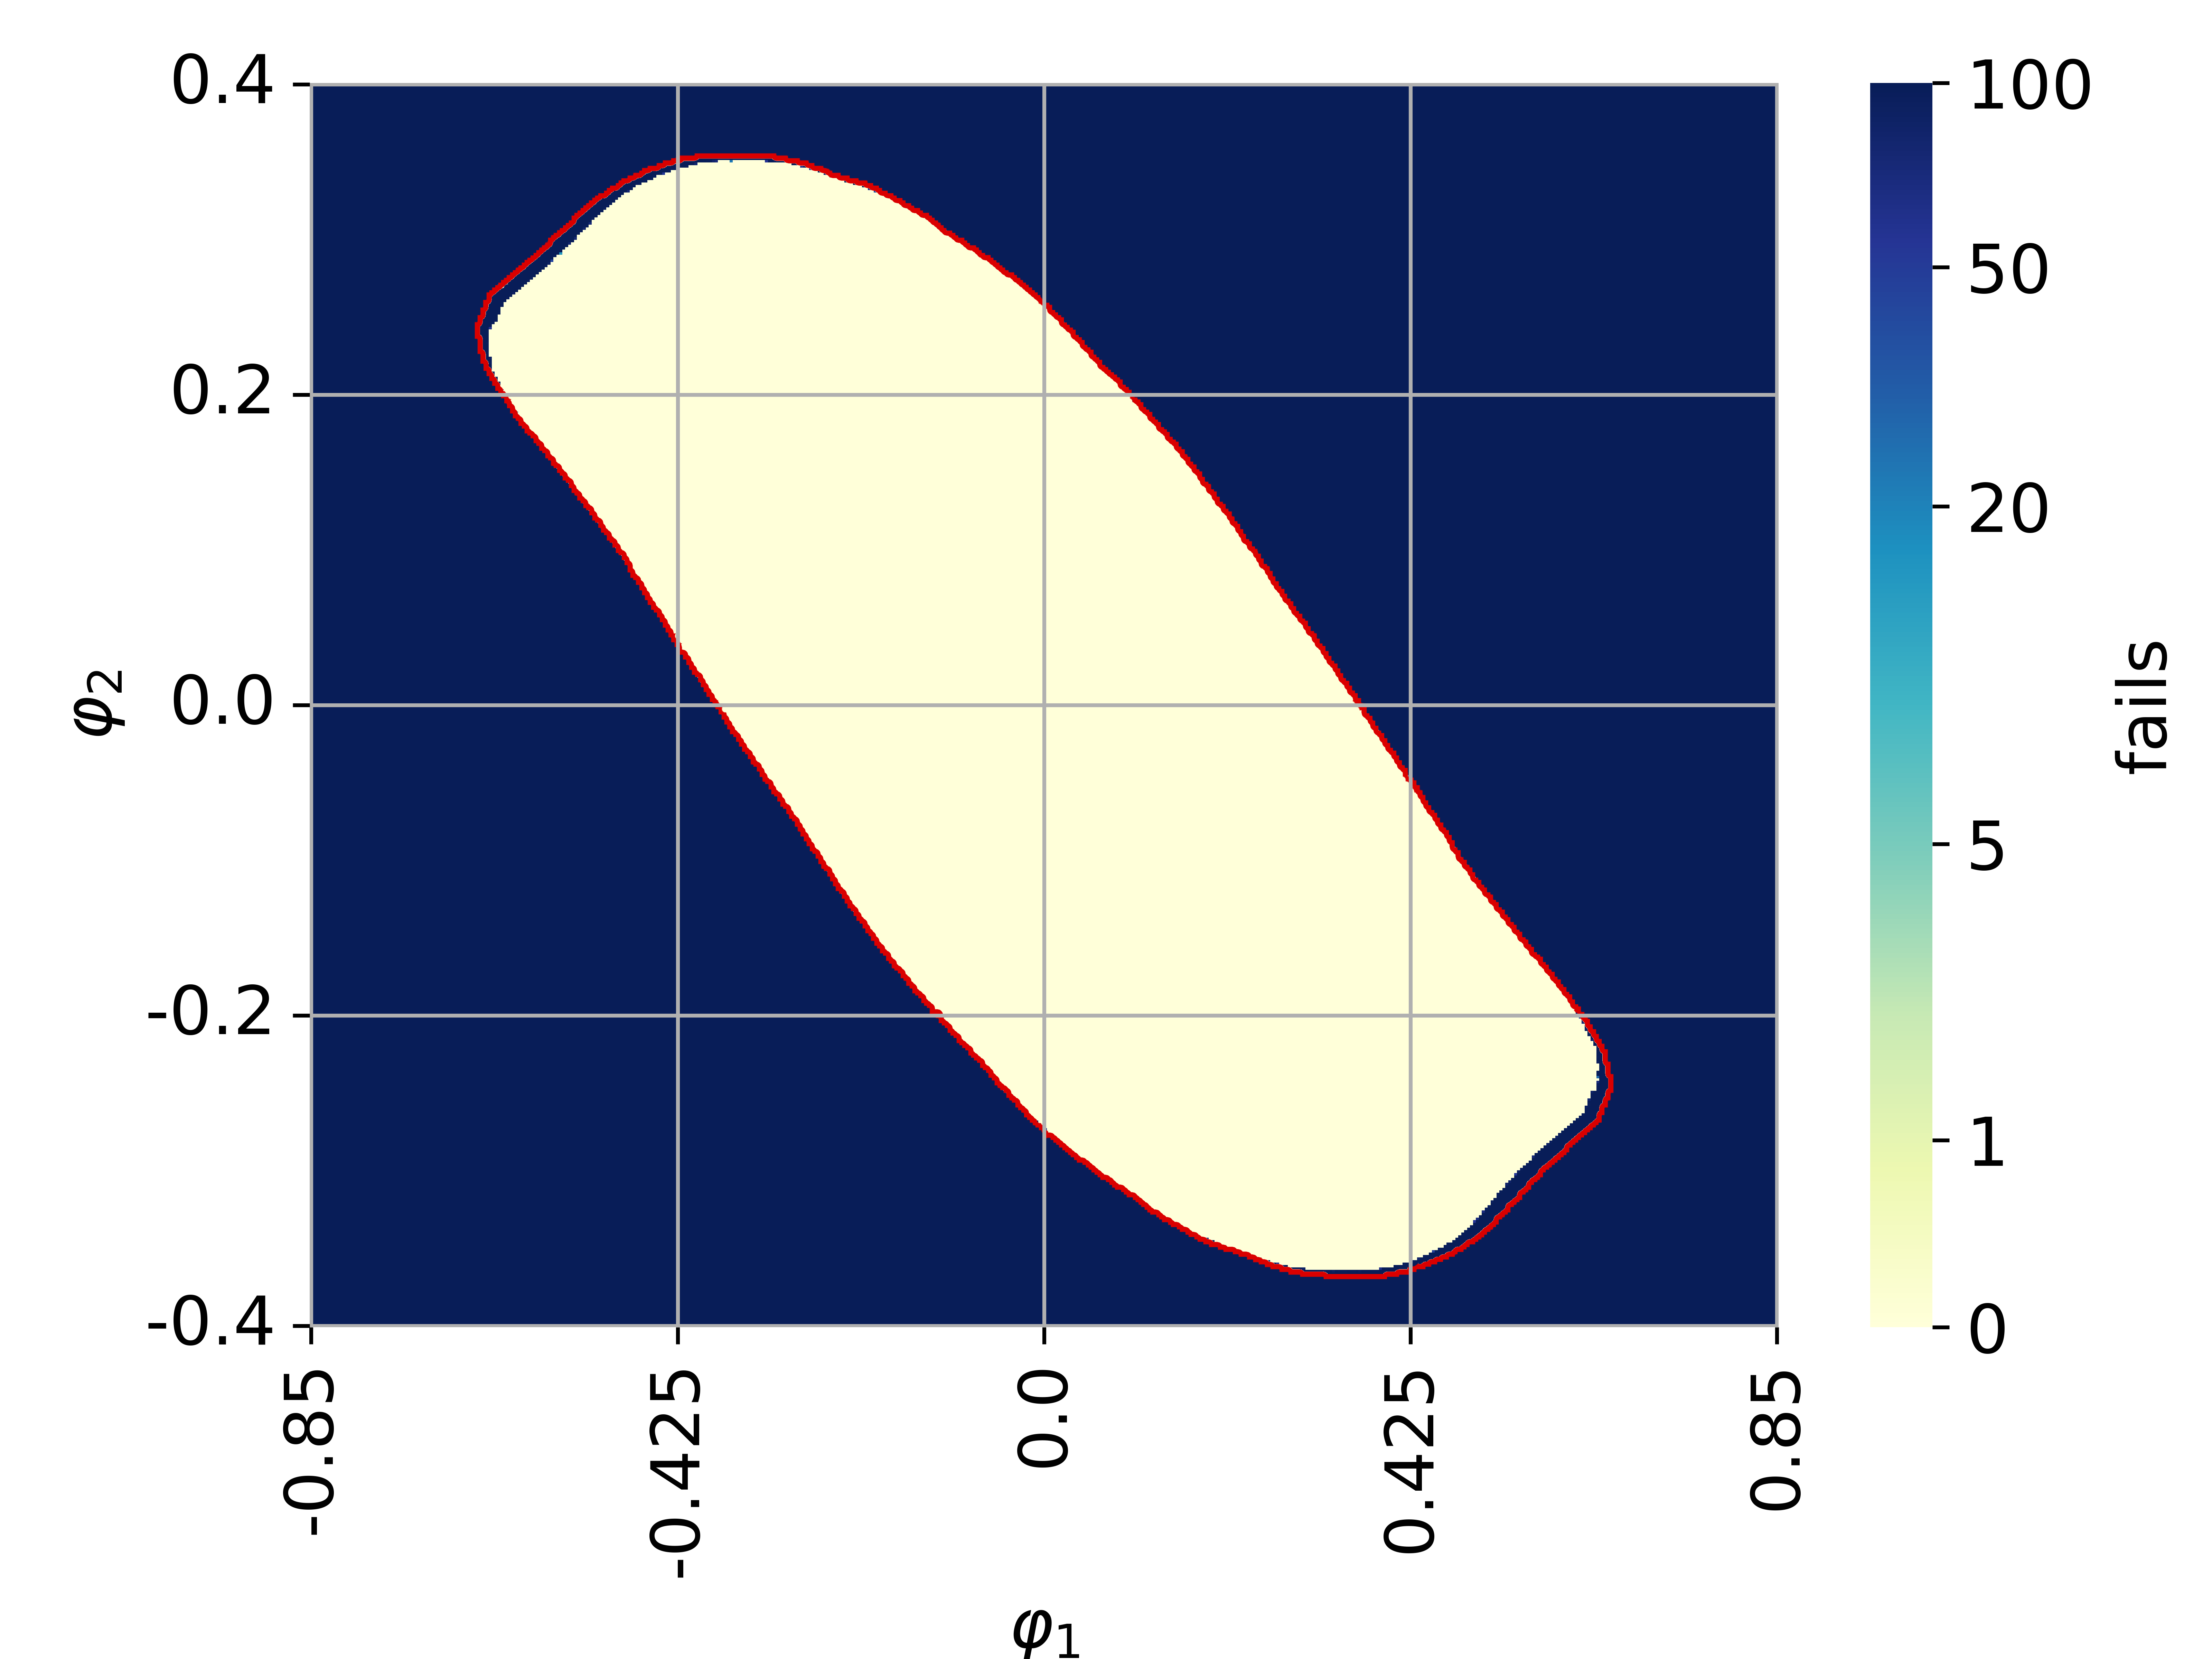
\includegraphics[width=\textwidth]{Figures/DP_friction_0.01.png}
         \label{fig: DP friction 0.01}
         \caption{}
     \end{subfigure}
     \hfill
     \begin{subfigure}[t]{0.32\textwidth}
         \centering
         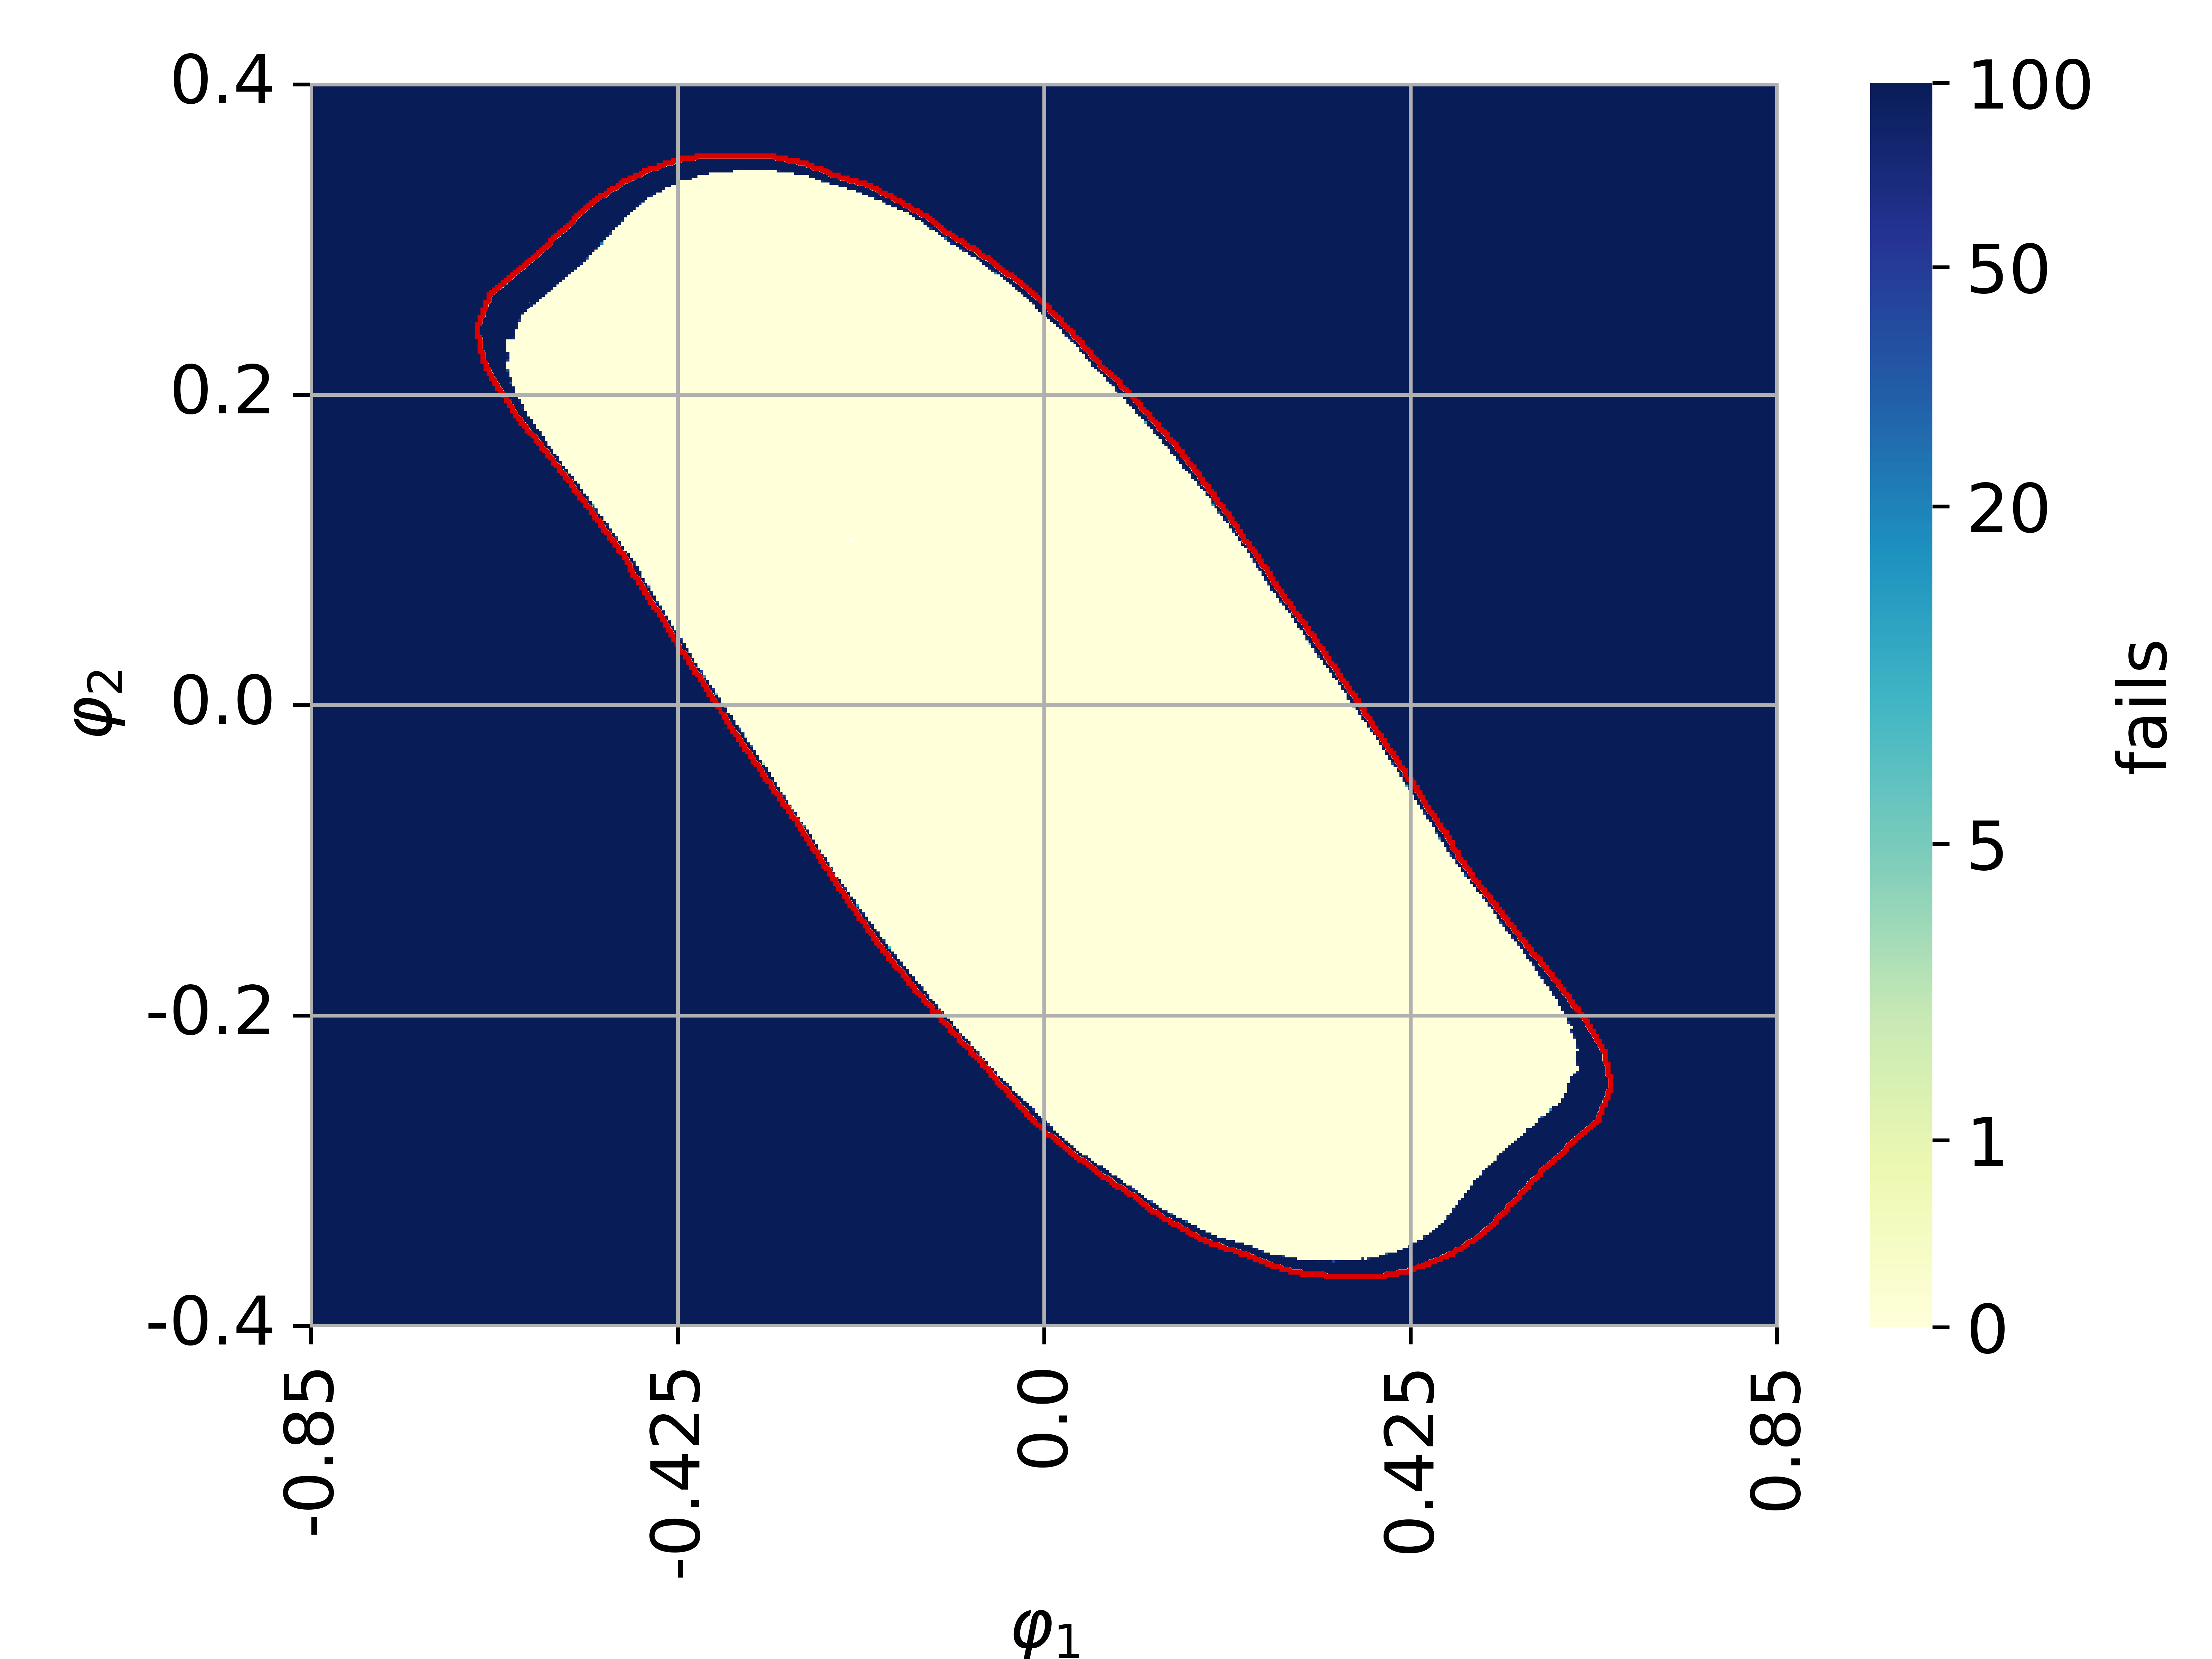
\includegraphics[width=\textwidth]{Figures/DP_friction_0.02.png}
         \label{fig: DP friction 0.02}
         \caption{}
     \end{subfigure}

     \caption{The stability zone for the double link system using the PPO agent, case 0. The red boundary corresponds to that depicted continuous control stability zone in Figure~\ref{fig: continuous vs discrete} (b). The environment parameters are modified as follows: (a) 1.1~$l$, (b) 1.2~$l$, (c) 1.1~$m$, (d) 1.2~$m$, (e) $f_rel$ = 0.01, and (f) $f_rel$ = 0.02.}
     \label{fig: agent impact on different environments}
 \end{figure}

The observations shows, that increasing the link length will cause the stability zone to expand, while not having the increase of the blind spots, as it was for the discrete control cases~\cite{manzl2023relrl}. Increasing the mass of the link doesn't provide any differences from the base model, so that we can state that up to the changes of 20$\%$ the model is independent from the link mass change.
Considering friction the stability zone becomes smaller within each increase of it, but the value of \( f_{\text{rel}} = 0.02 \) still provides us with the stable zone without causing the agent to fail in the original contour, as it was shown in~\cite{manzl2023relrl}. It can be concluded that the continuous control scheme is more suitable if friction is involved in the environment model simulation.

\subsection{RL training enhancement with CL} \label{subsec: RL training enhancement with CL}
To select the parameters needed for the CL implementation the research was conducted in the following fashion. At first, we determine which decay type is specifically the most performing for our particular task of pendulum stabilization. For this we have simulated 150 runs of 5 cases within the control values matrix of the form 
\(\begin{bmatrix} 1 & n \\ 0 & 0 \end{bmatrix}\), where \(n = 2, 4, 6, 8, 10\) and decay steps vector \(\begin{bmatrix} 0 \\ k \end{bmatrix}\), where \(k = 5000, 6000, \ldots, 10000\) to evaluate the performance across different control parameters. The results are presented in a form of a bar plot, which shows the number of agent successes for the whole dataset. It is shown, that the exponential decay type function, provides the best results of having 74$\%$ of successes across the dataset. Within this research conducted, in the next steps we have used this decay type to work with for the CL implementation. 

\begin{figure}[h]
	\centering
	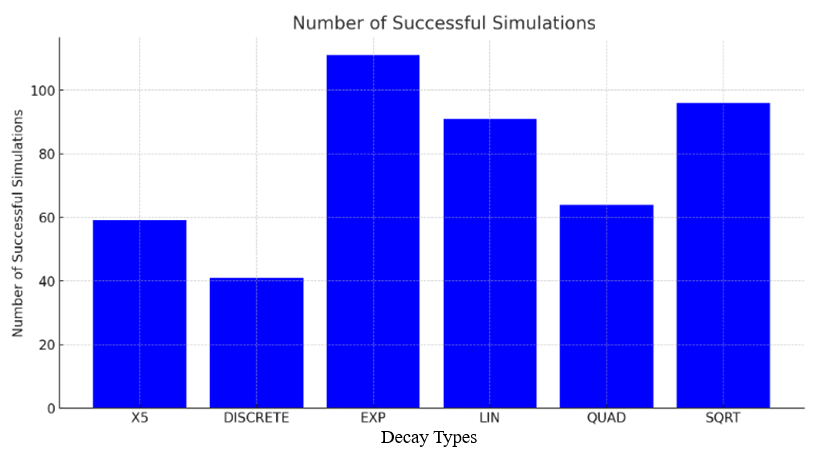
\includegraphics[width=10cm]{Figures/decay_types_results_comparison.png}
	\caption{}
	\label{fig: decay types comparison}
\end{figure}

